% Theory of Concurrency -- Lecture 6
% CCS, equational reasoning, bisimulation, and compiler optimisation.
% Based on the terminology, notation and visual language of lecture5.tex.
% Every diagram is editable TikZ. Speaker prompts are in \note{...}.
% Build slides: pdflatex -interaction=nonstopmode lecture6.tex (twice)
% Handout: pdflatex -jobname=lecture6_handout '\def\HANDOUT{1}\documentclass[t,11pt]{beamer}

% Lecture 6 follows the 4:3 Beamer style of the earlier course lectures.
\usepackage[T1]{fontenc}
\usepackage[utf8]{inputenc}
\usepackage{lmodern}
\usepackage{amsmath,amssymb,mathtools}
\usepackage{tikz}
\usetikzlibrary{arrows.meta,positioning,calc,fit,backgrounds}
\usepackage{array,booktabs}

\definecolor{LectureBlue}{RGB}{46,52,175}
\definecolor{BlockTitleLav}{RGB}{195,194,231}
\definecolor{BlockBodyLav}{RGB}{225,226,246}
\definecolor{SoftGray}{RGB}{115,115,115}
\useinnertheme[shadow=true]{rounded}
\setbeamercolor{normal text}{fg=black,bg=white}
\setbeamercolor{structure}{fg=LectureBlue}
\setbeamercolor{frametitle}{fg=LectureBlue,bg=white}
\setbeamercolor{block title}{fg=LectureBlue,bg=BlockTitleLav}
\setbeamercolor{block body}{fg=black,bg=BlockBodyLav}
\setbeamercolor{alerted text}{fg=LectureBlue}
\setbeamerfont{frametitle}{size=\Large,series=\mdseries}
\setbeamertemplate{blocks}[rounded][shadow=true]
\setbeamersize{text margin left=8pt,text margin right=8pt}
\setbeamertemplate{itemize items}[circle]
\setbeamertemplate{enumerate items}[circle]
\setlength{\parskip}{2pt}

\tikzset{
  state/.style={circle,draw=LectureBlue,thick,minimum size=9mm,inner sep=1pt,fill=white},
  event/.style={circle,draw=LectureBlue,thick,minimum size=10mm,inner sep=1pt,fill=white},
  flowarrow/.style={-{Latex[length=2mm]},thick,draw=black},
  dependency/.style={-{Latex[length=2mm]},thick,draw=LectureBlue},
  localbox/.style={draw=LectureBlue,rounded corners=2pt,inner sep=5pt},
  tag/.style={font=\small,fill=white,inner sep=1.4pt}
}
\newcommand{\domn}{\operatorname{dom}}
\newcommand{\Pref}{\operatorname{Pref}}
\newcommand{\lin}{\operatorname{Lin}}
\newcommand{\Sig}{\Sigma}
\newcommand{\wi}{\equiv_I}
\newcommand{\ind}{\mathrel{I}}
\newcommand{\dep}{\mathrel{D}}

\begin{document}

% =========================================================
\begin{frame}[plain]
  \vspace{1.10cm}
  \begin{center}
    {\huge\color{LectureBlue} Theory of Concurrency\par}
    \vspace{0.55cm}
    {\Large Lecture 6: Mazurkiewicz traces\par}
    \vspace{0.17cm}
    {\Large and Zielonka automata\par}
    \vspace{0.94cm}
    {\large Piotr Hofman\par}
  \end{center}
\end{frame}

\begin{frame}{Plan}
  \begin{enumerate}
    \item Problems with linear semantics.
    \item Histories.
    \item Independence relations and Mazurkiewicz traces.
    \item Dependence graphs, partial orders and Foata normal form.
    \item Trace-closed languages and their specifications.
    \item Zielonka automata and the distributed realisation theorem.
  \end{enumerate}
  \vspace{0.4cm}
  \begin{block}{Central question}
    How can we describe and implement concurrent behaviour without fixing an arbitrary order between independent events?
  \end{block}
\end{frame}


\section{Interleaving versus concurrency}

\begin{frame}{Two independent actions in an LTS}
  \begin{block}{Two local variables}
    Initially $(x,y)=(0,0)$. Action $a$ sets $x:=1$ and action $b$ sets $y:=1$.
  \end{block}
  \vspace{0.1cm}
  \begin{center}
  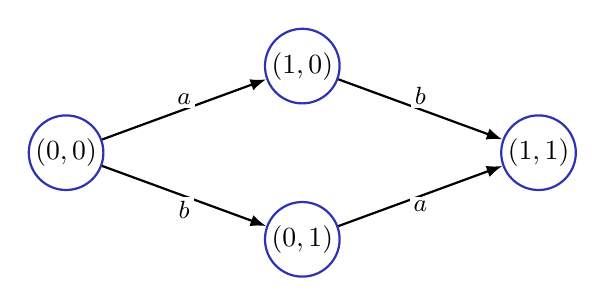
\begin{tikzpicture}[x=1cm,y=1cm]
    \node[state] (s0) at (-3,0) {$(0,0)$};
    \node[state] (sa) at (0,1.1) {$(1,0)$};
    \node[state] (sb) at (0,-1.1) {$(0,1)$};
    \node[state] (sf) at (3,0) {$(1,1)$};
    \draw[flowarrow] (s0) -- node[tag,above] {$a$} (sa);
    \draw[flowarrow] (s0) -- node[tag,below] {$b$} (sb);
    \draw[flowarrow] (sa) -- node[tag,above] {$b$} (sf);
    \draw[flowarrow] (sb) -- node[tag,below] {$a$} (sf);
  \end{tikzpicture}
  \end{center}
  \begin{block}{Two paths, the same result}
    Both $ab$ and $ba$ are executions, and both end in $(1,1)$.
  \end{block}
\end{frame}

\begin{frame}{What does an ordinary trace record?}
  \begin{block}{Interleaving semantics}
    A run of an LTS produces a word: a \emph{total order} of the actions executed.
    \[
      ab\neq ba \qquad \text{as words in }\Sigma^*.
    \]
  \end{block}
  \begin{block}{But in the preceding example}
    Neither action affects the other one's enabledness or result. The difference between $ab$ and $ba$ is only their scheduling order.
  \end{block}
  \vspace{0.12cm}
  \centering\large We want to retain necessary order, but forget irrelevant order.
\end{frame}

\begin{frame}{Interleaving explosion}
  \begin{block}{Two sequential processes}
    One process performs $a_1,a_2,\ldots,a_m$ in order; another performs $b_1,b_2,\ldots,b_n$ in order. Cross-process actions are independent.
  \end{block}
  \[
    \text{number of interleavings}=\binom{m+n}{m}.
  \]
  \begin{center}
  \begin{tabular}{c|c|c}
  First process & Second process & Interleavings\\ \hline
  $m=2$ & $n=2$ & $6$\\
  $m=4$ & $n=4$ & $70$\\
  $m=10$ & $n=10$ & $184\,756$
  \end{tabular}
  \end{center}
\end{frame}

\begin{frame}{Fairness and linearisation}
  \begin{block}{Two concurrent loops}
    Consider one process that repeatedly emits $a$, and another that repeatedly emits $b$.
    \[
    P_1: a\,a\,a\,\ldots
    \qquad \text{||}\qquad
    P_2: b\,b\,b\,\ldots
    \]
    These are independent threads of activity, not a single sequential program.
  \end{block}
  \begin{block}{A natural fairness requirement}
    The specification 
    \[
    \mathbf{G}(a\Rightarrow \mathbf{F}b) \text{does not hold for the linearisation }\ a,a,a,\cdots.
    \]
    
   \end{block}
  \begin{block}{Why this matters}
    Fairness is a property of the run as a concurrent system, not of an arbitrary total order chosen by the scheduler. Linear semantics can therefore hide behavioural defects or impose artificial ordering constraints.
  \end{block}
\end{frame}


\begin{frame}{Causality}
  \begin{block}{Independence versus dependence}
    Two events are \emph{independent} if neither one enables, disables, nor changes the effect of the other. They may be executed in either order without changing the observable outcome.
  \end{block}
  \begin{block}{Causal order}
    If one event is required to occur before another because it influences its result or enables it, then the first is a \emph{cause} of the second. This gives a partial order, not a total one.
  \end{block}
  \begin{center}
  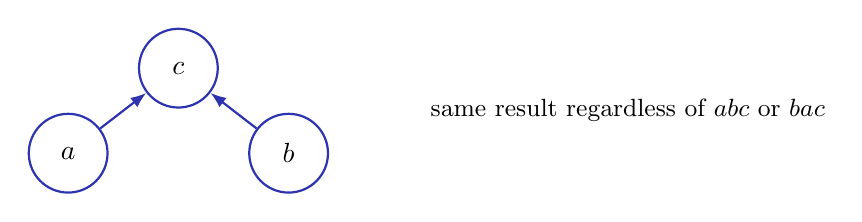
\begin{tikzpicture}[x=1.4cm,y=.9cm]
    \node[event] (a) at (0,0) {$a$};
    \node[event] (b) at (2,0) {$b$};
    \node[event] (c) at (1,1.2) {$c$};
    \draw[dependency] (a) -- (c);
    \draw[dependency] (b) -- (c);
    \node[font=\small,anchor=west] at (3.2,0.6) {same result regardless of $abc$ or $bac$};
  \end{tikzpicture}
  \end{center}
 
\end{frame}


\begin{frame}{Why linear semantics is not enough}
  \begin{block}{A scheduler chooses an order, but not necessarily a causal one}
    An execution of a concurrent system is often represented as a word
    \[
      a_1a_2\cdots a_n.
    \]
  \end{block}
  \begin{block}{Problems}
    \begin{itemize}
      \item The word order records arbitrary scheduling choices, not essential causality.
      \item Fairness may require that a process is eventually scheduled, even if its actions are not the next ones in a fixed linearisation.
      \item Exponential blow-up appears because independent actions generate many equivalent serialisations.
    \end{itemize}
  \end{block}
  \centering\large The semantics should keep only the order that matters for behaviour.
\end{frame}

\begin{frame}{Distributed logs (Another problem)}
  \begin{block}{Problem with logging}
    In distributed systems, each machine writes its local events with its own clock. A global log is often assembled later by merging timestamps, but different clocks may drift and messages may be delayed or reordered.
  \end{block}
  \begin{block}{Example: Patriot missile failure 1991}
    \begin{itemize}
      \item After 100 hours, the radar clock drifted by 0.34 seconds.
      \item This small error shifted the tracked position of a Scud by roughly 500 meters.
      \item The missile missed its target; 28 soldiers were killed.
    \end{itemize}
  \end{block}

\end{frame}

% \begin{frame}{Histories}
%   \begin{block}{Processes and their alphabets}
%     Let $P=\{p_1,p_2,p_3\}$, with local alphabets
%     \[
%       \Sigma_{p_1}=\{a,c\},\quad \Sigma_{p_2}=\{b,c\},\quad \Sigma_{p_3}=\{d\}.
%     \]
%     An action shared by processes is communication: they synchronize by executing that same action. Here $c$ is one event involving both $p_1$ and $p_2$.
%   \end{block}
%   \begin{center}
%   \begin{tikzpicture}[x=.9cm,y=.7cm]
%     \draw[black,thick] (-2,1.2) -- (2,1.2);
%     \draw[black,thick] (-2,0.2) -- (2,0.2);
%     \draw[black,thick] (-2,-0.8) -- (2,-0.8);
%     \node[font=\small,anchor=east] at (-2,1.2) {$p_1$};
%     \node[font=\small,anchor=east] at (-2,0.2) {$p_2$};
%     \node[font=\small,anchor=east] at (-2,-0.8) {$p_3$};
%     \node[event,minimum size=8mm] (p1a) at (-0.6,1.2) {$a$};
%     \node[event,minimum size=8mm] (p1c) at (1.3,1.2) {$c$};
%     \node[event,minimum size=8mm] (p2b) at (-0.6,0.2) {$b$};
%     \node[event,minimum size=8mm] (p2c) at (1.3,0.2) {$c$};
%     \node[event,minimum size=8mm] (p3d) at (0.3,-0.8) {$d$};
%     \draw[dependency] (p1a) -- (p1c);
%     \draw[dependency] (p2b) -- (p2c);
%     \draw[thick,dashed] (p1c) -- node[tag,right,font=\scriptsize] {same event} (p2c);
%   \end{tikzpicture}
%   \end{center}

% \end{frame}

% \begin{frame}{When is swapping actions incorrect?}
%   \begin{block}{Shared variable}
%     Let $a$ assign $x:=1$ and $b$ assign $x:=2$.
%   \end{block}
%   \[
%   \begin{aligned}
%     x=0&\xrightarrow{a}x=1\xrightarrow{b}x=2,\\[5pt]
%     x=0&\xrightarrow{b}x=2\xrightarrow{a}x=1.
%   \end{aligned}
%   \]
%   \begin{block}{Dependence matters}
%     The order of $a$ and $b$ changes the outcome. They cannot be declared independent.
%   \end{block}
%\end{frame}


% \begin{frame}{Histories (Approach 1)}


% \begin{block}{What should be dependnet?}
% Actions in the same process are dependent. For them, we have causality relation.
% \end{block}

%    \begin{block}{Dependence and independence}
%     Actions are dependent iff their process domains intersect; disjoint domains mean independence. Thus $a$ and $b$ are independent, as is $d$ from $a,b,c$.
%   \end{block}

% \end{frame}


\begin{frame}{Histories (Approach 1)}
\begin{block}{Assumptions:}
\begin{enumerate}
 \item We have $k$ processes running in parallel. 
 \item Each action of the process$_i$ has a unique name in $\Sigma_i$.
 \item They communicate via rendezvous.
 \item If $a$ belongs to the alphabets of a few systems then all
 of them perform it synchronously.  
\end{enumerate}
\end{block}

\visible<2->{
\begin{block}{}
We consider a monoid $M=\Sigma_1^*\times \Sigma_2^*\times
\ldots \Sigma_k^*$ with concatenation defined via coordinates $(u_1,u_2,\ldots, u_k)+(w_1,w_2,\ldots, w_k)=
(u_1 w_1,u_2 w_2,\ldots, u_k w_k)$.
\end{block}
}
\visible<3->{
\begin{block}{}
Let $\Sigma=\Sigma_1\cup\Sigma_2\cup\ldots \Sigma_k$. For 
$a\in \Sigma$ we define $u_a\in M$ as $(x_1,x_2,\ldots,x_k)$
where $x_i=\varepsilon$ if $a\not\in \Sigma_i$ and
$x_i=a$ if $a\in \Sigma_i$. We call the set of $u_a$ elementary histories.
\end{block}
}


\end{frame}




\begin{frame}{Histories}

\begin{block}{The history is}
a submonoid of $M$ generated by elementary histories.
\end{block}
\visible<2->{
\begin{block}{Projection $\pi_i$}
For a word $w\in \Sigma^*$ its projection $\pi_i$ is a
word $w_i\in \Sigma_i^*$ obtained from $w$ by removing letters 
not in $\Sigma_i$.
\end{block}
}
\visible<3->{
\begin{block}{Projection $\pi$}
For a word $w\in \Sigma^*$ its projection $\pi$ is an element of the monoid $M$
$(\pi_1(w),\pi_2(w),\ldots,\pi_k(w))$.
\end{block}
}
\visible<4->{
\begin{block}{Mathematical structure of histories}
\begin{itemize}
 \item Monoid structure.
 \item Projections goes form strings to the monoid of histories.
\end{itemize}
\end{block}
}

\end{frame}





% =========================================================


% =========================================================
\section{Mazurkiewicz traces}

\newcommand{\Ind}{I}
\newcommand{\Dep}{D}


\begin{frame}{Independence and dependence alphabets (Approach 2)}
  \begin{block}{Definition}
    A \emph{concurrent alphabet} is $(\Sigma,I)$, where $\Sigma$ is finite and
    \[
       \Ind\subseteq\Sigma\times\Sigma
    \]
    is a \textbf{symmetric, irreflexive} independence relation.
  \end{block}
  \begin{block}{Dependence relation}
    \[
      D=(\Sigma\times\Sigma)\setminus I.
    \]
    Dependence is symmetric and reflexive.
  \end{block}
  \vspace{0.1cm}
  We read $a\ind b$ as ``$a$ and $b$ may commute'', and $a\dep b$ as ``their order must be retained''.
\end{frame}

\begin{frame}{A running dependence alphabet}
  \[
    \Sigma=\{a,b,c\},\qquad I=\{(a,b),(b,a)\}.
  \]
  \begin{center}
  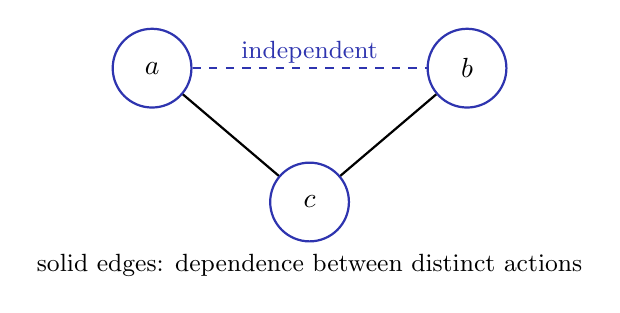
\begin{tikzpicture}[scale=1]
    \node[event] (a) at (-2,0) {$a$};
    \node[event] (b) at (2,0) {$b$};
    \node[event] (c) at (0,-1.7) {$c$};
    \draw[LectureBlue,thick,dashed] (a) -- node[tag,above] {independent} (b);
    \draw[thick] (a) -- (c);
    \draw[thick] (b) -- (c);
    \node[font=\small] at (0,-2.5) {solid edges: dependence between distinct actions};
  \end{tikzpicture}
  \end{center}
  \begin{block}{Important distinction}
    $a\ind b$, while $a\dep c$ and $b\dep c$. Dependence need not be transitive; every action also depends on itself.
  \end{block}
\end{frame}

\begin{frame}{Swapping independent neighbours}
  \begin{block}{Elementary equivalence}
    If $a\ind b$, then for every $u,v\in\Sigma^*$,
    \[
      uabv \;\longleftrightarrow\; ubav.
    \]
    Let $\equiv_I$ be the equivalence relation generated by these swaps.
  \end{block}
  \begin{block}{Example: $I=\{(a,b),(b,a)\}$}
    \[
    \underbrace{abc\equiv_I bac}_{\text{swap }a,b},
    \qquad
    \underbrace{abc\not\equiv_I acb}_{\text{cannot swap }b,c}.
    \]
  \end{block}
  Swaps act on \emph{adjacent} positions; a sequence of swaps may be needed.
\end{frame}

\begin{frame}{Mazurkiewicz traces}
  \begin{block}{Definition}
    A \emph{Mazurkiewicz trace} is an equivalence class of words under $\equiv_I$:
    \[
      [w]_I=\{v\in\Sigma^*:v\equiv_I w\}.
    \]
  \end{block}
  \begin{block}{Our example}
    For $I=\{(a,b),(b,a)\}$,
    \[
      [abc]_I=\{abc,bac\},\qquad [acb]_I=\{acb\}.
    \]
  \end{block}
  \vspace{0.25cm}
  A trace represents an execution \emph{up to permutations of independent actions}.
\end{frame}

\begin{frame}{Why traces form a monoid}
  \begin{block}{Congruence property}
    Swapping independent neighbours remains valid inside larger words:
    \[
      u\equiv_Iu',\quad v\equiv_Iv'
      \quad\Longrightarrow\quad uv\equiv_Iu'v'.
    \]
  \end{block}
  \begin{block}{Trace monoid}
    \[
      M(\Sigma,I)=\Sigma^*/{\equiv_I},\qquad
      [u]_I\cdot[v]_I=[uv]_I.
    \]
    The empty word $\varepsilon$ induces the identity element $[\varepsilon]_I$.
  \end{block}
  \vspace{0.15cm}
  Concatenation of traces is well-defined, independently of the chosen word representatives.
\end{frame}

\begin{frame}{Two extreme forms of independence}
  \begin{block}{No independent distinct actions: $I=\varnothing$}
    No swaps are allowed. Every trace consists of one word:
    \[
      M(\Sigma,\varnothing)=\Sigma^*.
    \]
  \end{block}
  \begin{block}{All distinct actions independent}
    $I=\{(a,b):a\neq b\}$. Words are equivalent exactly when each letter occurs equally often.
    \[
      abc\equiv_I bca\equiv_I cab.
    \]
    The trace remembers only the numbers of occurrences of actions.
  \end{block}
  Most concurrent alphabets lie between these extremes.
\end{frame}

\begin{frame}{From word languages to trace languages}
  \begin{block}{Quotient map}
    \[
       q:\Sigma^*\longrightarrow M(\Sigma,I),\qquad q(w)=[w]_I.
    \]
    A word language $L\subseteq\Sigma^*$ induces the trace language
    \[
       q(L)=\{[w]_I:w\in L\}.
    \]
  \end{block}

\end{frame}

%=================
\section{Comparison of traces and histories}

\begin{frame}{}

\begin{block}{}
By $u \div a$ we mean right cancellation of $a$ from $u$. For $u$ beeing a string
it is defined as follows:
$$ u \div a = \begin{cases}
\varepsilon \ for\ u=\varepsilon,\\
v\ for\ u=va\\
(v\div a)b \ for \ u=vb\ where \ b\neq a
\end{cases}  $$
\end{block}
 
\begin{lemma}
  $u \equiv w \implies u \div a \equiv w \div a$ for any $a\in \Sigma$.
\end{lemma}

\visible<2->{ 
\begin{block}{}
A dependency morphism w.r.t. $D$ is any homomorphism from the monoid of strings over $\Sigma$
on to another monoid such that
\begin{enumerate}
\item[A1] $\phi(w)=\phi(\varepsilon) \implies w=\varepsilon;$
\item[A2]$(a,b)\in\Ind \implies \phi(ab)=\phi(ba);$
\item[A3] $\phi(ua)=\phi(v) \implies \phi(u)=\phi(v\div a);$
\item[A4] $\phi(ua)=\phi(vb)\land a\neq b \implies (a,b)\in \Ind$
\end{enumerate} 
\end{block}
}
\end{frame}



\begin{frame}{}
We want to prove $3$ theorems.

\begin{theorem}
Let $\phi$ and $\psi$ are two dependency morphism going from $\Sigma^*$ to monoids $M$ and $N$. Then $M$ and $N$ are isomorphic. 
\end{theorem}

\visible<2->{
\begin{lemma}
Let $\phi$ be a dependency morphism, $u,v\in \Sigma^*$ $a,b\in \Sigma$. If $\phi(ua)=\phi(vb)$ and $a\neq b$ then there exists $w\in \Sigma^*$ such that $\phi(u)=\phi(wb)$ and $\phi(v)=\phi(wa)$.
\end{lemma}
}

\visible<3->{
\begin{theorem}
Canonical homomorphism of string into Mazurkiewicz traces is a dependency morphism.  
\end{theorem}
}

\visible<4->{
\begin{theorem}
Canonical homomorphism of string into histories is a dependency morphism.  
\end{theorem}
}
\end{frame}





% =========================================================
\section{Partial-order representation}

\begin{frame}{From total orders to partial orders}
  \begin{center}
  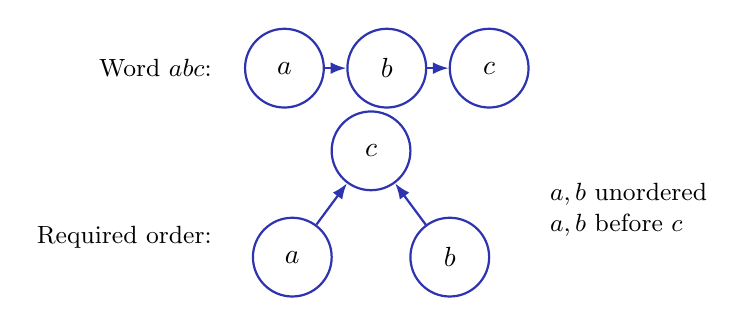
\begin{tikzpicture}[x=1cm,y=1cm]
    \node[font=\small,anchor=east] at (-2.5,0.6) {Word $abc$:};
    \node[event] (wa) at (-1.7,.6) {$a$};
    \node[event] (wb) at (-.4,.6) {$b$};
    \node[event] (wc) at (.9,.6) {$c$};
    \draw[dependency] (wa) -- (wb);
    \draw[dependency] (wb) -- (wc);
    \node[font=\small,anchor=east] at (-2.5,-1.55) {Required order:};
    \node[event] (pa) at (-1.6,-1.8) {$a$};
    \node[event] (pb) at (.4,-1.8) {$b$};
    \node[event] (pc) at (-.6,-.45) {$c$};
    \draw[dependency] (pa) -- (pc);
    \draw[dependency] (pb) -- (pc);
    \node[font=\small,align=left,anchor=west] at (1.55,-1.2) {$a,b$ unordered\\$a,b$ before $c$};
  \end{tikzpicture}
  \end{center}
  \begin{block}{Idea}
    A word imposes an order on \emph{all} positions. A dependence graph keeps only the order forced by dependent actions.
  \end{block}
\end{frame}

\begin{frame}{Dependence graph of a word}
  \begin{block}{Construction}
    Let $w=a_1a_2\cdots a_n$. Create a distinct event vertex for each position:
    Add an edge $i\to j$ whenever
    \[
       i<j\quad\text{and}\quad (a_i,a_j)\in D.
    \]
    Take the reflexive transitive closure to obtain the order $\leq_w$.
  \end{block}
  \begin{block}{Important}
    Vertices are \textbf{occurrences}, not action names. In particular, two occurrences of the same action are ordered because $(a,a)\in D$.
  \end{block}
\end{frame}

\begin{frame}{Dependence graph: $abc$}
  \[
      I=\{(a,b),(b,a)\},\qquad w=abc.
  \]
  \begin{center}
  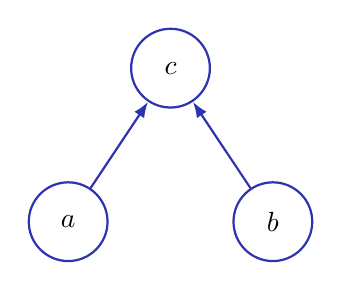
\begin{tikzpicture}[x=1cm,y=1cm]
    \node[event] (a) at (-1.3,-1.4) {$a$};
    \node[event] (b) at (1.3,-1.4) {$b$};
    \node[event] (c) at (0,0.55) {$c$};
    \draw[dependency] (a) -- (c);
    \draw[dependency] (b) -- (c);
    \node[font=\small] at (0,-2.0) {%The Hasse diagram of the dependence order
    };
  \end{tikzpicture}
  \end{center}
  \begin{block}{Linearizations}
    The labelled partial order has exactly two linearizations:
    \[
       \lin(E_w,\leq_w,\lambda)=\{abc,bac\}.
    \]
  \end{block}
\end{frame}

\begin{frame}{Independent labels can still be ordered}
  \[
     I=\{(a,b),(b,a)\},\qquad w=acb.
  \]
  \begin{center}
  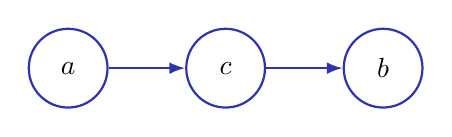
\begin{tikzpicture}
    \node[event] (a) at (-2,0) {$a$};
    \node[event] (c) at (0,0) {$c$};
    \node[event] (b) at (2,0) {$b$};
    \draw[dependency] (a) -- (c);
    \draw[dependency] (c) -- (b);
  \end{tikzpicture}
  \end{center}
  \begin{block}{Transitive causality}
    Although $a\ind b$, the order contains $a<c<b$ because both actions depend on $c$.
  \end{block}
  \vspace{0.2cm}
  Independence of \emph{action labels} does not guarantee that two particular \emph{occurrences} are unordered.
\end{frame}

\begin{frame}{Fundamental characterisation of traces}
  \begin{block}{Theorem}
    For finite words $u,v\in\Sigma^*$,
    \[
       u\equiv_Iv
       \quad\Longleftrightarrow\quad
       \text{their labelled dependence posets are isomorphic}.
    \]
  \end{block}
  \begin{block}{Proof idea: $\Rightarrow$}
    Swapping adjacent independent events preserves every order constraint between dependent occurrences.
  \end{block}
  \begin{block}{Proof idea: $\Leftarrow$}
    Any two linear extensions of a finite poset are connected by adjacent swaps of incomparable events. In a dependence poset, incomparable events have independent labels.
  \end{block}
\end{frame}

\begin{frame}{Lexicographic normal form}
  \begin{block}{Choose an order on the alphabet}
    Fix a total order, for example $a<b<c$. Each trace contains finitely many words, so it has a unique lexicographically least representative.
    \[
      \operatorname{lexmin}([w]_I)
      =\min_{\mathrm{lex}}\{v\in\Sigma^*:v\equiv_Iw\}.
    \]
  \end{block}
  \begin{block}{Example}
    With $I=\{(a,b),(b,a)\}$,
    \[
       [abc]_I=\{abc,bac\},\qquad
       \operatorname{lexmin}([abc]_I)=abc.
    \]
  \end{block}
  The chosen word is canonical, but it is still a \emph{total order}: it does not display which events could have happened concurrently.
\end{frame}

\begin{frame}{Foata normal form: concurrent layers}
  \begin{block}{Canonical representation}
    Repeatedly take all minimal events of the dependence poset, record them as one layer, and remove them. Every layer consists of pairwise independent actions.
  \end{block}
  \[
      w=abcabc,\qquad I=\{(a,b),(b,a)\}.
  \]
  \begin{center}
  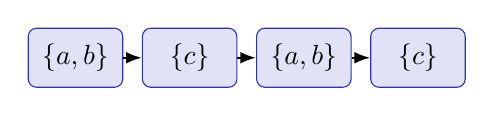
\begin{tikzpicture}[x=1.45cm,y=.75cm]
    \node[draw=LectureBlue,rounded corners=3pt,fill=BlockBodyLav,minimum width=1.2cm,minimum height=.75cm] (k0) at (0,0) {$\{a,b\}$};
    \node[draw=LectureBlue,rounded corners=3pt,fill=BlockBodyLav,minimum width=1.2cm,minimum height=.75cm] (k1) at (1,0) {$\{c\}$};
    \node[draw=LectureBlue,rounded corners=3pt,fill=BlockBodyLav,minimum width=1.2cm,minimum height=.75cm] (k2) at (2,0) {$\{a,b\}$};
    \node[draw=LectureBlue,rounded corners=3pt,fill=BlockBodyLav,minimum width=1.2cm,minimum height=.75cm] (k3) at (3,0) {$\{c\}$};
    \draw[flowarrow] (k0) -- (k1);
    \draw[flowarrow] (k1) -- (k2);
    \draw[flowarrow] (k2) -- (k3);
  \end{tikzpicture}
  \end{center}
  \begin{block}{Foata normal form}
    \[
       \{a,b\}\;\{c\}\;\{a,b\}\;\{c\}.
    \]
    These layers are uniquely determined by a finite trace.
  \end{block}
\end{frame}

\begin{frame}{Foata layers are not time slots}
  \[
    \Sigma=\{a,b,c\},\qquad I=\{(a,b),(b,a),(b,c),(c,b)\}.
  \]
  Thus $a\dep c$, while $b$ is independent of both $a$ and $c$.
  \begin{block}{One trace, two linearizations}
    The words $abc$ and $acb$ differ only by swapping the independent actions $b,c$.
    Their dependence order has just one constraint: $a<c$.
  \end{block}
  \begin{center}
    \[
      \operatorname{Foata}(abc)=\operatorname{Foata}(acb)
      =\{a,b\}\;\{c\}.
    \]
  \end{center}
  \begin{block}{How to read the layers}
    The layers give events their dependence depth; they are not strict time slots.
    Here $b$ is in the first layer but may occur after $c$, as the linearization $acb$ shows.
  \end{block}
\end{frame}


\begin{frame}{Foata form and lexicographic form}
  \begin{center}
  \begin{tabular}{>{\raggedright\arraybackslash}p{.27\textwidth}|>{\raggedright\arraybackslash}p{.30\textwidth}|>{\raggedright\arraybackslash}p{.30\textwidth}}
    & \textbf{Lexicographic} & \textbf{Foata}\\ \hline
    Representation & One chosen word & A sequence of concurrent layers\\
    Captures concurrency & No; serialises a trace & Yes; independent events can share a layer\\
    Canonical? & Yes, after fixing an alphabet order & Yes, from the dependence order\\
    Useful for & Comparing or storing traces as words & Seeing causal depth and available parallelism
  \end{tabular}
  \end{center}
  \begin{block}{Same trace, different emphasis}
    For $[abc]_I=\{abc,bac\}$ with $a\ind b$, the lexicographic form is $abc$, while the Foata form is $\{a,b\}\{c\}$.
  \end{block}
\end{frame}


\begin{frame}{What information does a trace preserve?}
  \begin{block}{Preserved}
    Event occurrences, action labels, and the ordering constraints induced by dependence.
  \end{block}
  \begin{block}{Forgotten}
    The chosen interleaving of incomparable events. A trace does not record physical durations or a schedule.
  \end{block}
  \begin{block}{Not represented by one trace}
    Branching choices between different possible executions of an entire system.
  \end{block}
\end{frame}

% =========================================================
\section{Trace languages}



\begin{frame}{Trace-closed languages}
  \begin{block}{Definition}
    A language $L\subseteq\Sigma^*$ is \emph{$I$-closed} (or \emph{trace-closed}) if
    \[
      u\in L\ \text{and}\ u\equiv_Iv
      \quad\Longrightarrow\quad v\in L.
    \]
    Equivalently, $uabv\in L$ iff $ubav\in L$ whenever $a\ind b$.
  \end{block}
  \begin{block}{Example}
    Let $\Sigma=\{a,b,c\}$, with $a\ind b$ and both dependent on $c$. Let
    \[
      A=(a+b)^*,\qquad R=AaAbA+AbAaA,\qquad L=(Rc)^*A.
    \]
    $R$ consists of words containing both letters; each $c$ closes one such block. Swapping neighbouring $a,b$ preserves membership in $L$.
  \end{block}
\end{frame}

\begin{frame}{A requirement that is not trace-closed}
  \[
     \Sigma=\{a,b\},\qquad a\ind b,\qquad L=\{ab\}.
  \]
  \begin{block}{Problem}
    $ab\in L$, but $ba\notin L$, although $ab\equiv_Iba$.
  \end{block}
  \[
    q^{-1}\bigl(q(L)\bigr)=\{ab,ba\}\neq L.
  \]
  \begin{block}{Interpretation}
    The specification explicitly requires $a$ before $b$, so these two actions cannot simultaneously be treated as independent for this requirement.
  \end{block}
\end{frame}

\begin{frame}{Why an LTS should satisfy diamonds}
  \begin{block}{Commutation property}
    For independent $a,b$, whenever
    $s\xrightarrow{a}s_1\xrightarrow{b}t$,
    there must be some $s_2$ with
    $s\xrightarrow{b}s_2\xrightarrow{a}t$.
  \end{block}
  \begin{center}
  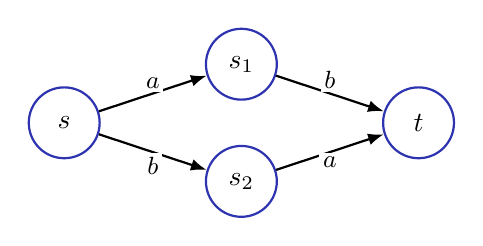
\begin{tikzpicture}[x=1cm,y=.62cm]
    \node[state] (s) at (-2.25,0) {$s$};
    \node[state] (sa) at (0,1.2) {$s_1$};
    \node[state] (sb) at (0,-1.2) {$s_2$};
    \node[state] (t) at (2.25,0) {$t$};
    \draw[flowarrow] (s) -- node[tag,above] {$a$} (sa);
    \draw[flowarrow] (s) -- node[tag,below] {$b$} (sb);
    \draw[flowarrow] (sa) -- node[tag,above] {$b$} (t);
    \draw[flowarrow] (sb) -- node[tag,below] {$a$} (t);
  \end{tikzpicture}
  \end{center}
  \begin{block}{Consequence}
    If this replacement is always possible along runs, the finite trace language of the LTS is $I$-closed.
  \end{block}
\end{frame}

\begin{frame}{From regular specifications to distributed machines}
  \begin{block}{Finite-state specification}
    Regularity means that a finite automaton can recognise the word language $L\subseteq\Sigma^*$. This is a finite-state description of the allowed executions.
  \end{block}
  \begin{block}{Concurrency-respecting specification}
    If $L$ is $I$-closed, acceptance depends on the trace, not on which order independent actions happened to take.
  \end{block}
  \begin{block}{Implementation question}
    Can such a specification be implemented with finite local states, so each action accesses only the processes that participate in it?
  \end{block}
  \centering\textbf{Zielonka's theorem says yes for every regular, $I$-closed language.}
\end{frame}

% =========================================================
\section{Zielonka automata}

\begin{frame}{Distributed alphabets}
  \begin{block}{Definition}
    Let $P$ be a finite set of processes. A \emph{distributed alphabet} provides
    \[
       \domn:\Sigma\longrightarrow 2^P\setminus\{\varnothing\}.
    \]
    The set $\domn(a)$ contains exactly the processes that participate in $a$.
  \end{block}
  \begin{center}
    \begin{tabular}{c|c|l}
      action & domain & meaning\\ \hline
      $a$ & $\{p\}$ & local action of $p$\\
      $b$ & $\{q\}$ & local action of $q$\\
      $c$ & $\{p,q\}$ & synchronization of $p$ and $q$
    \end{tabular}
  \end{center}
  \[
      a\ind b\quad\Longleftrightarrow\quad \domn(a)\cap\domn(b)=\varnothing.
  \]
\end{frame}

\begin{frame}{Why process domains explain independence}
  \begin{center}
  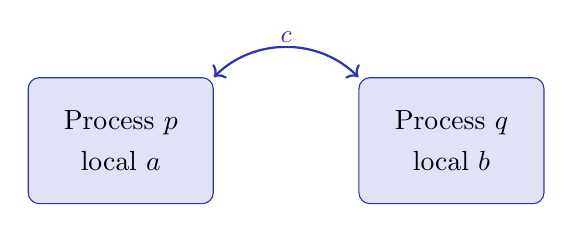
\begin{tikzpicture}[x=1cm,y=1cm]
    \node[draw=LectureBlue,rounded corners,fill=BlockBodyLav,minimum width=2.35cm,minimum height=1.6cm,align=center] (p) at (-2.1,0) {Process $p$\\[3pt]local $a$};
    \node[draw=LectureBlue,rounded corners,fill=BlockBodyLav,minimum width=2.35cm,minimum height=1.6cm,align=center] (q) at (2.1,0) {Process $q$\\[3pt]local $b$};
    \draw[LectureBlue,thick,<->] (p.north east) to[out=45,in=135] node[tag,above] {$c$} (q.north west);
  \end{tikzpicture}
  \end{center}
  \begin{block}{Local and shared actions}
    $a$ changes only the state of $p$, while $b$ changes only the state of $q$. Action $c$ involves both processes and can coordinate their states.
  \end{block}
  \vspace{0.15cm}
  Disjoint process domains give a structural reason for the commutation of actions.
\end{frame}

\begin{frame}{Zielonka automata: local states}
  \begin{block}{Global configuration}
    Each process $p\in P$ has a finite local state space $Q_p$ and initial state $q_p^0$. A global configuration is a tuple
    \[
        (q_p)_{p\in P}\in\prod_{p\in P}Q_p.
    \]
  \end{block}
  \begin{block}{Action semantics}
    An action $a$ reads and updates \emph{only} the states of processes in $\domn(a)$. All other local states remain unchanged.
  \end{block}
  \vspace{0.18cm}
  A shared action is one atomic synchronization step of all its participating processes.
\end{frame}

\begin{frame}{Formal definition of a Zielonka automaton}
  \begin{block}{Deterministic finite asynchronous automaton}
    A Zielonka automaton consists of finite local state sets $(Q_p)_{p\in P}$, an initial tuple $q^0$, a set of accepting global states
    \[
      F\subseteq\prod_{p\in P}Q_p,
    \]
    and, for each $a\in\Sigma$, a \emph{partial} local update function
    \[
      \delta_a:\prod_{p\in\domn(a)}Q_p
      \rightharpoonup\prod_{p\in\domn(a)}Q_p.
    \]
  \end{block}
  \begin{block}{Reading a word}
    Execute its actions from $q^0$ when their local updates are defined. A word is accepted if the final global tuple belongs to $F$.
  \end{block}
\end{frame}

\begin{frame}{A two-process Zielonka automaton}
  \begin{block}{Local states and initial configuration}
    Processes $p$ and $q$ each have local state space $\{0,1\}$, with initial state $0$.
    Thus the initial global configuration is $(0,0)$.
  \end{block}
  \begin{center}
  \begin{tabular}{c|c|l}
    action & domain & partial local update\\ \hline
    $a$ & $\{p\}$ & $0\mapsto1$ on $p$\\
    $b$ & $\{q\}$ & $0\mapsto1$ on $q$\\
    $c$ & $\{p,q\}$ & $(1,1)\mapsto(0,0)$
  \end{tabular}
  \end{center}
  \begin{block}{Reading the updates}
    Actions $a$ and $b$ are enabled only when their process is in state $0$; they are independent.
    The synchronization $c$ is enabled only when both processes are in state $1$ and resets both.
  \end{block}
  Every global state is accepting. The next slide shows the resulting global LTS.
\end{frame}

\begin{frame}{Global LTS of the Zielonka automaton}
  \begin{center}
  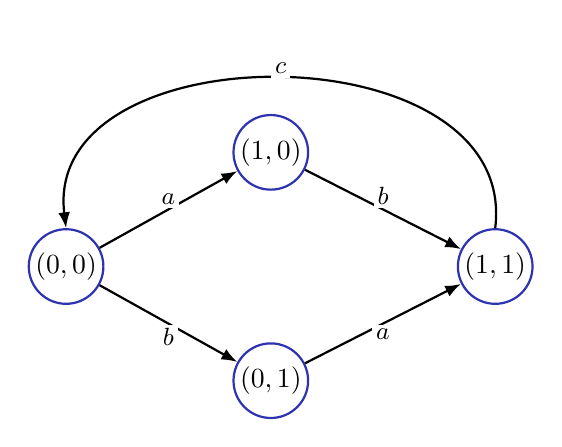
\begin{tikzpicture}[x=1cm,y=1cm]
    \node[state] (s0) at (-3,0) {$(0,0)$};
    \node[state] (sa) at (-.4,1.45) {$(1,0)$};
    \node[state] (sb) at (-.4,-1.45) {$(0,1)$};
    \node[state] (sf) at (2.45,0) {$(1,1)$};
    \draw[flowarrow] (s0) -- node[tag,above] {$a$} (sa);
    \draw[flowarrow] (s0) -- node[tag,below] {$b$} (sb);
    \draw[flowarrow] (sa) -- node[tag,above] {$b$} (sf);
    \draw[flowarrow] (sb) -- node[tag,below] {$a$} (sf);
    \draw[flowarrow] (sf.north) to[out=83,in=97,looseness=1.2] node[tag,above] {$c$} (s0.north);
  \end{tikzpicture}
  \end{center}
  \begin{block}{Global view, local implementation}
    The diagram is an ordinary LTS, but its transitions are generated from local updates and one shared synchronization.
  \end{block}
\end{frame}

\begin{frame}{The language recognised by the example}
  \begin{block}{Accept all reachable global states}
    Take $F=Q_p\times Q_q$. Then the accepted language consists of valid prefixes of rounds with one $a$, one $b$, and a closing $c$:
    \[
       L=\Pref\bigl(((ab+ba)c)^*\bigr).
    \]
  \end{block}
  \begin{center}
  \begin{tabular}{l|l}
    accepted & not accepted\\ \hline
    $\varepsilon,\ a,\ b,\ ab,\ ba$ & $c$\\
    $abc,\ bac,\ abcabc$ & $acb,\ aabc$
  \end{tabular}
  \end{center}
  \begin{block}{Trace closure}
    Every exchange of adjacent $a,b$ preserves acceptance: $abc$ and $bac$ are two linearizations of one accepted trace.
  \end{block}
\end{frame}

\begin{frame}{Independence is built into the automaton}
  \begin{block}{Disjoint local updates commute}
    If $\domn(a)\cap\domn(b)=\varnothing$, the two updates read and modify disjoint coordinates.
    \[
       q\xrightarrow{a}q_1\xrightarrow{b}q'
       \quad\Longleftrightarrow\quad
       q\xrightarrow{b}q_2\xrightarrow{a}q'.
    \]
  \end{block}
  \begin{block}{Consequence}
    Every word accepted by a Zielonka automaton can be replaced by any $I$-equivalent word without changing the final global state. Its language is $I$-closed.
  \end{block}
  \vspace{0.15cm}
  This follows from the architecture, not from a separately imposed commutation axiom.
\end{frame}

\begin{frame}{Zielonka's theorem}
  \begin{block}{Theorem (Zielonka, 1987)}
    Fix a finite distributed alphabet $(\Sigma,\domn)$ and its induced independence relation $I$.

    If a language $L\subseteq\Sigma^*$ is
    \begin{itemize}
      \item regular, and
      \item $I$-closed,
    \end{itemize}
    then $L$ is recognised by a \textbf{finite deterministic Zielonka automaton} over this distributed alphabet.
  \end{block}
  \begin{block}{Conversely}
    Every language recognised by a finite Zielonka automaton (with global final states) is regular and $I$-closed.
  \end{block}
\end{frame}



\begin{frame}{What does Zielonka's theorem say?}
  \begin{block}{Specification}
    A centralised finite automaton can specify a global behaviour language, provided it is closed under the independence relation.
  \end{block}
  \begin{block}{Implementation}
    There exists a finite automaton with separate local states: every action uses only the local states of its participating processes.
  \end{block}
  \begin{block}{Limit of the result}
    The theorem is an expressiveness result. It does \emph{not} promise a small distributed implementation. The construction and its size bounds are nontrivial.
  \end{block}
\end{frame}

\begin{frame}{Why local projections are not enough}
  \begin{block}{Two processes and a trace-closed language}
    Let $\domn(a)=\{p\}$, $\domn(b)=\{q\}$, and $\domn(c)=\{p,q\}$, so $a\ind b$. Consider
    \[
      L=\{acb,\ bca\}.
    \]
    This language is $I$-closed: the independent actions $a,b$ are never adjacent in either word.
  \end{block}
  \begin{block}{Project onto each process}
    \[
      \pi_p(L)=\{ac,ca\},\qquad \pi_q(L)=\{cb,bc\}.
    \]
    A construction accepting whenever both local projections are accepted also accepts $w=abc$, since
    \[
      \pi_p(w)=ac\in\pi_p(L),\qquad \pi_q(w)=bc\in\pi_q(L).
    \]
    But $abc\notin L$.
  \end{block}
\end{frame}

\begin{frame}{The missing information: correlation}
  \begin{block}{What the projections forget}
    In $acb$, process $p$ performs $ac$ while $q$ performs $cb$. In $bca$, they perform $ca$ and $bc$. Separate projections also allow the mixed combination $ac$ with $bc$, producing the spurious word $abc$.
  \end{block}
  \begin{block}{Scope of the counterexample}
    This refutes the rule ``accept iff every process accepts its projection,'' not Zielonka's theorem. In this example, local states can retain which projected word occurred, and a suitable set of \emph{global} accepting tuples can accept the two intended combinations while rejecting the mixed one.
  \end{block}
  \begin{block}{Why the theorem is nontrivial}
    A distributed automaton must preserve enough information about which local behaviours can occur together. The theorem guarantees a finite construction that does so; simply recognising each projection independently does not.
  \end{block}
\end{frame}





\begin{frame}{Proof}
Blackbord. 
\end{frame}



\begin{frame}{References}
  \begin{thebibliography}{10}
    \bibitem{Zielonka87}
    W. Zielonka.
    \newblock \emph{Notes on finite asynchronous automata}.
    \newblock RAIRO -- Theoretical Informatics and Applications, 21(2):99--135, 1987.

    \bibitem{BookTraces}
    V. Diekert and G. Rozenberg (eds.).
    \newblock \emph{The Book of Traces}.
    \newblock World Scientific, 1995.

    \bibitem{BaierKatoen}
    C. Baier and J.-P. Katoen.
    \newblock \emph{Principles of Model Checking}.
    \newblock MIT Press, 2008.
  \end{thebibliography}
\end{frame}

\end{document}
'
\ifdefined\HANDOUT
  \documentclass[handout,aspectratio=169,11pt]{beamer}
\else
  \documentclass[aspectratio=169,11pt]{beamer}
\fi
\usepackage[T1]{fontenc}
\usepackage[utf8]{inputenc}
\usepackage{lmodern}
\usepackage{amsmath,amssymb,mathtools,booktabs,array}
\usepackage{tikz}
\usetikzlibrary{arrows.meta,positioning,calc,fit,backgrounds}
\usepackage{appendixnumberbeamer}
\usefonttheme{professionalfonts}
\definecolor{Ink}{HTML}{20283A}
\definecolor{Indigo}{HTML}{43458A}
\definecolor{Pale}{HTML}{F0F0F8}
\definecolor{Teal}{HTML}{167B79}
\definecolor{PaleTeal}{HTML}{EAF5F3}
\definecolor{Warn}{HTML}{A4433C}
\definecolor{PaleWarn}{HTML}{FBF0EE}
\definecolor{Muted}{HTML}{626B7C}
\setbeamercolor{normal text}{fg=Ink,bg=white}
\setbeamercolor{structure}{fg=Indigo}
\setbeamercolor{frametitle}{fg=Indigo}
\setbeamercolor{title}{fg=Indigo}
\setbeamercolor{block title}{fg=Indigo,bg=Pale}
\setbeamercolor{block body}{fg=Ink,bg=Pale}
\setbeamercolor{block title example}{fg=Teal,bg=PaleTeal}
\setbeamercolor{block body example}{fg=Ink,bg=PaleTeal}
\setbeamercolor{block title alerted}{fg=Warn,bg=PaleWarn}
\setbeamercolor{block body alerted}{fg=Ink,bg=PaleWarn}
\setbeamertemplate{blocks}[rounded][shadow=false]
\setbeamertemplate{navigation symbols}{}
\setbeamertemplate{bibliography item}[text]
\setbeamersize{text margin left=8mm,text margin right=8mm}
\setbeamerfont{frametitle}{size=\Large,series=\bfseries}
\setbeamerfont{block title}{size=\normalsize,series=\bfseries}
\setbeamerfont{footnote}{size=\scriptsize}
\setbeamertemplate{itemize item}{\small\raise0.2ex\hbox{\textbullet}}
\setbeamertemplate{itemize subitem}{\tiny\raise0.2ex\hbox{\textbullet}}
\setbeamercovered{invisible}
\setbeameroption{hide notes}
\newif\ifinbackup
\inbackupfalse
\setbeamertemplate{headline}{\color{Indigo}\rule{\paperwidth}{0.5mm}}
\setbeamertemplate{footline}{%
  \leavevmode\hbox{%
    \begin{beamercolorbox}[wd=.79\paperwidth,ht=3.5mm,dp=2mm,leftskip=8mm]{normal text}%
      \color{Muted}\scriptsize Theory of Concurrency\enspace/\enspace Lecture 6\enspace/\enspace\insertsectionhead
    \end{beamercolorbox}%
    \begin{beamercolorbox}[wd=.21\paperwidth,ht=3.5mm,dp=2mm,rightskip=8mm plus1fil]{normal text}%
      \hfill\color{Muted}\scriptsize\ifinbackup Backup\enspace\fi\insertframenumber\,/\,\inserttotalframenumber
    \end{beamercolorbox}%
  }}
\setlength{\abovedisplayskip}{6pt}
\setlength{\belowdisplayskip}{6pt}
\newcommand{\step}[1]{\xrightarrow{#1}}
\newcommand{\wstep}[1]{\xRightarrow{#1}}
\newcommand{\wb}{\mathrel{\approx_{\mathrm w}}}
\newcommand{\rwb}{\mathrel{\approx_{\mathrm{rw}}}}
\newcommand{\nil}{\mathbf 0}
\newcommand{\blockact}[2]{\operatorname{block}_{#1}(#2)}
\newcommand{\Source}[1]{\par\vspace{2mm}{\scriptsize\color{Muted}#1\par}}
\newcommand{\Takeaway}[1]{\begin{exampleblock}{}#1\end{exampleblock}}
\newcommand{\optional}{\textcolor{Muted}{\scriptsize OPTIONAL}\quad}
\newcommand{\Store}[2]{\langle #1,\,#2\rangle}
\newcommand{\state}[1]{\mathsf{#1}}
\newcommand{\code}[1]{\texttt{#1}}
\newcommand{\smallrule}{\color{Pale}\rule{\textwidth}{0.45pt}}
\tikzset{
  >=Latex,
  st/.style={circle,draw=Indigo,line width=.7pt,fill=white,minimum size=7.5mm,inner sep=1pt,font=\small},
  terminal/.style={st,draw=Muted},
  trans/.style={->,line width=.85pt,draw=Ink},
  tauedge/.style={trans,draw=Teal},
  newedge/.style={trans,draw=Warn,line width=1.1pt},
  rel/.style={dashed,draw=Teal,line width=.9pt},
  lab/.style={font=\small,fill=white,inner sep=1.2pt},
  tinylabel/.style={font=\scriptsize,fill=white,inner sep=1pt},
  panel/.style={rounded corners=2mm,fill=Pale,draw=none,inner sep=4mm}
}
\title{CCS and algebraic proofs}
\subtitle{From bisimulation to compiler optimisation}
\author{Piotr Hofman}
\institute{Theory of Concurrency}
\date{}

\begin{document}

\section{A proof-oriented perspective}
% 1
\begin{frame}[plain]
  \vspace{9mm}
  {\color{Muted}\large THEORY OF CONCURRENCY\par}
  \vspace{6mm}
  {\color{Indigo}\LARGE\bfseries CCS and algebraic proofs\par}
  \vspace{3mm}
  {\Large From bisimulation to compiler optimisation\par}
  \vspace{8mm}
  {\large Lecture 6\quad\textcolor{Muted}{Piotr Hofman}\par}
  \vfill
  \begin{beamercolorbox}[sep=3mm,wd=\textwidth]{block body}
    How do we justify replacing one program fragment with another?\\[1mm]
    \textbf{Define behaviour}\quad $\to$\quad \textbf{prove equivalence}\quad $\to$\quad \textbf{use congruence}.
  \end{beamercolorbox}
  \vspace{3mm}
\end{frame}
\note{90 min. Previous lecture introduced bisimulation and rooted congruence; this lecture uses them as tools rather than redefining them.}

% 2
\begin{frame}{What we already know from Lecture 5}
  \begin{columns}[T,onlytextwidth]
    \begin{column}{.47\textwidth}
      \begin{block}{Semantics}
        SOS rules define an LTS for every process expression.\\[2mm]
        Strong and weak bisimulations compare transition systems.
      \end{block}
    \end{column}
    \begin{column}{.47\textwidth}
      \begin{block}{Composition}
        A congruence permits substitution inside a context.\\[2mm]
        Rootedness matters when internal steps meet choice.
      \end{block}
    \end{column}
  \end{columns}
  \vspace{4mm}
  \Takeaway{Today: make the relation \emph{useful} for calculations and correctness proofs.}
  \note{Ask: Is weak bisimilarity alone a congruence for choice? No. Do not spend time re-proving it.}
\end{frame}

% 3
\begin{frame}{Two ways to prove a transformation correct}
  \begin{center}
  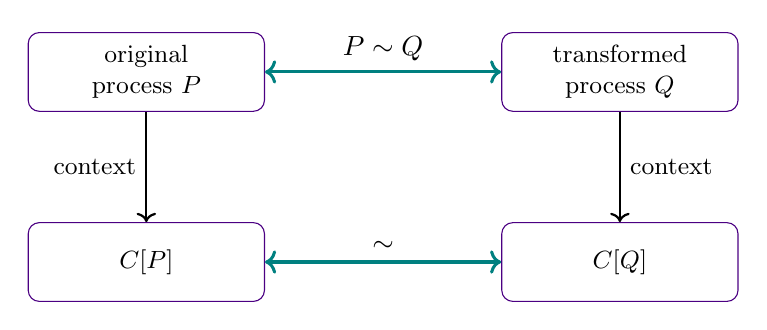
\begin{tikzpicture}[node distance=7mm and 10mm, every node/.style={font=\small}]
    \node[draw=Indigo,rounded corners,minimum width=3.0cm,minimum height=1.0cm,align=center] (a) {original\\process $P$};
    \node[draw=Indigo,rounded corners,minimum width=3.0cm,minimum height=1.0cm,align=center,right=3.0cm of a] (b) {transformed\\process $Q$};
    \draw[<->,line width=1.1pt,draw=Teal] (a)--node[above,font=\normalsize] {$P\sim Q$} (b);
    \node[below=14mm of a,draw=Indigo,rounded corners,minimum width=3.0cm,minimum height=1.0cm,align=center] (ac) {$C[P]$};
    \node[below=14mm of b,draw=Indigo,rounded corners,minimum width=3.0cm,minimum height=1.0cm,align=center] (bc) {$C[Q]$};
    \draw[->,line width=.8pt] (a)--node[left] {context} (ac);
    \draw[->,line width=.8pt] (b)--node[right] {context} (bc);
    \draw[<->,line width=1.1pt,draw=Teal] (ac)--node[above,font=\normalsize] {$\sim$} (bc);
  \end{tikzpicture}
  \end{center}
  \vspace{2mm}
  \begin{columns}[T,onlytextwidth]
    \begin{column}{.48\textwidth}\textbf{Equational method:} rewrite $P$ using sound algebraic laws.\end{column}
    \begin{column}{.48\textwidth}\textbf{Relational method:} exhibit a bisimulation between $P$ and $Q$.\end{column}
  \end{columns}
  \note{The diagram uses strong bisim, a congruence for our CCS constructors. Later replace it by rooted weak bisim for hidden internal work.}
\end{frame}

\section{CCS as an algebra}
% 4
\begin{frame}{A fragment of CCS}
  \begin{block}{Syntax}
  \[
    P ::= \nil \mid \alpha.P \mid P+P \mid P\parallel P
       \mid \blockact{H}{P},\qquad \alpha\in\Sigma\cup\{\tau\}.
  \]
  \end{block}
  \renewcommand{\arraystretch}{1.35}
  \begin{tabular}{@{}p{.25\textwidth}p{.67\textwidth}@{}}
    $\alpha.P$ & Prefix: first $\alpha$, then $P$.\\
    $P+Q$ & Alternative initial transitions (nondeterministic choice).\\
    $P\parallel Q$ & Interleaving plus synchronisation of $a$ with $\bar a$.\\
    $\blockact{H}{P}$ & Block labels in $H$; $\tau$ is never blocked.
  \end{tabular}
  \Source{Same notation as Lecture 5; standard CCS restriction of a channel corresponds to blocking both $a$ and $\bar a$.}
  \note{This is recursion-free CCS with explicit action-blocking notation retained from L5. No fairness assumption.}
\end{frame}

% 5
\begin{frame}{One rule, three kinds of transitions}
  \begin{block}{Interleaving}
    \[
      \frac{P\step{\alpha}P'}{P\parallel Q\step{\alpha}P'\parallel Q}
      \qquad
      \frac{Q\step{\beta}Q'}{P\parallel Q\step{\beta}P\parallel Q'}
    \]
  \end{block}
  \begin{exampleblock}{Communication}
    \[
      \frac{P\step{a}P'\quad Q\step{\bar a}Q'}
      {P\parallel Q\step{\tau}P'\parallel Q'}
    \]
  \end{exampleblock}
  \Takeaway{A handshake is \emph{possible}, not compulsory, until exposed actions are blocked.}
  \note{The three derivations are exactly the new parallel SOS rules of Lecture 5. Emphasise that prefix, choice and blocking were already introduced.}
\end{frame}

% 6
\begin{frame}{Parallel composition: three initial moves}
  \[
     P=a.\nil\parallel\bar a.\nil
  \]
  \centering
  \begin{tikzpicture}[x=1cm,y=1cm]
    \node[st] (p) at (0,1.2) {$P$};
    \node[st] (l) at (-3,-.5) {$\nil\parallel\bar a.\nil$};
    \node[st] (r) at (3,-.5) {$a.\nil\parallel\nil$};
    \node[terminal] (d) at (0,-.9) {$\nil\parallel\nil$};
    \draw[trans] (p) -- node[lab,above left] {$a$} (l);
    \draw[trans] (p) -- node[lab,above right] {$\bar a$} (r);
    \draw[tauedge] (p) -- node[lab,left] {$\tau$} (d);
  \end{tikzpicture}
  \par\vspace{2mm}
  \Takeaway{The system exposes $a$, exposes $\bar a$, \emph{or} communicates internally.}
  \note{Make students name the three transitions. The diagram deliberately omits later transitions from the left and right derivatives.}
\end{frame}

% 7
\begin{frame}{Blocking forces an internal handshake}
  \[
     S=\blockact{H}{a.b.\nil\parallel\bar a.c.\nil},
     \qquad H=\{a,\bar a\}.
  \]
  \vspace{2mm}
  \centering
  \begin{tikzpicture}[x=1cm,y=1cm]
    \node[st,minimum size=9mm] (s) at (0,0) {$S$};
    \node[st,minimum size=9mm] (t) at (4,0) {$T$};
    \draw[tauedge] (s)--node[lab,above] {$\tau$}(t);
    \node[font=\small,text=Muted,below=5mm of t,align=center] {$T=\blockact{H}{b.\nil\parallel c.\nil}$};
  \end{tikzpicture}
  \vspace{3mm}
  \begin{block}{Why only one transition?}
    $a$ and $\bar a$ are blocked individually; their synchronisation produces $\tau$, which survives.
  \end{block}
  \note{Assume all visible names a,b,c are distinct and b,c do not form a complementary pair. This avoids unnecessary handshake complications in T.}
\end{frame}

% 8
\begin{frame}{When may we write $P=Q$ in CCS calculations?}
  \begin{block}{Sound reading of an equation}
    Write $P\equiv Q$ for a proved equation; interpret it as
    \[
      P\equiv Q \quad\Longrightarrow\quad P\sim Q.
    \]
  \end{block}
  \begin{exampleblock}{Why use strong bisimilarity here?}
    It preserves the branching structure and is a congruence for all constructors in our fragment.
  \end{exampleblock}
  \Takeaway{Equational proofs are compressed bisimulation proofs.}
  \note{One may write P\sim Q in calculations directly; distinguish syntactic equality from a sound equational proof system.}
\end{frame}

% 9
\begin{frame}{Four basic equations for choice}
  \begin{align*}
    P+Q &\sim Q+P &&\text{(commutativity)}\\[2mm]
    (P+Q)+R &\sim P+(Q+R) &&\text{(associativity)}\\[2mm]
    P+P &\sim P &&\text{(idempotence)}\\[2mm]
    P+\nil &\sim P &&\text{(zero)}
  \end{align*}
  \vspace{3mm}
  \Takeaway{The same four equations hold for all $P,Q,R$, including processes with $\tau$.}
  \Source{A complete axiomatisation of strong bisimilarity for finite Basic CCS ($\nil$, prefix, choice). See van Glabbeek, \emph{Modelling Concurrent Systems}.}
  \note{One can justify idempotence by relating P+P to P and their derivatives. No law a.(P+Q)=a.P+a.Q is included!}
\end{frame}

% 10
\begin{frame}{Useful laws for parallelism and blocking}
  \begin{align*}
    P\parallel\nil &\sim P,\\[3mm]
    \blockact{H}{P+Q}&\sim \blockact{H}{P}+\blockact{H}{Q}.
  \end{align*}
  \begin{block}{Blocking a prefix}
    \[
      \blockact{H}{\alpha.P}\sim
      \begin{cases}
        \alpha.\blockact{H}{P},&\alpha\notin H,\\
        \nil,&\alpha\in H.
      \end{cases}
    \]
  \end{block}
  \Takeaway{All equations preserve \emph{strong} bisimilarity.}
  \note{H is a set of visible labels, not containing tau; so tau always takes the first branch. The P||0 law follows from a simple coinductive relation.}
\end{frame}

% 11
\begin{frame}{A tempting \emph{false} law}
  \[
  \blockact{H}{P\parallel Q}
  \quad\not\sim\quad
  \blockact{H}{P}\parallel\blockact{H}{Q}.
  \]
  \vspace{2mm}
  \begin{block}{Counterexample}
    \[
      P=a.\nil,\quad Q=\bar a.\nil,\quad H=\{a,\bar a\}.
    \]
    \[
      \underbrace{\blockact{H}{a.\nil\parallel\bar a.\nil}}_{\step{\tau}\text{ enabled}}
      \qquad\qquad
      \underbrace{\blockact{H}{a.\nil}\parallel\blockact{H}{\bar a.\nil}}_{\text{deadlocked}}.
    \]
  \end{block}
  \Takeaway{Blocking \emph{after} composing preserves the possibility of synchronisation.}
  \note{This is the central anti-law. Students often expect restriction to distribute over every constructor.}
\end{frame}

% 12
\begin{frame}{The CCS expansion theorem}
  \vspace{1mm}
  Suppose $P=\sum_{i\in I}\alpha_i.P_i$ and $Q=\sum_{j\in J}\beta_j.Q_j$.
  \begin{block}{Expand the initial moves of $P\parallel Q$}
    \vspace{-2mm}
    \begin{align*}
    P\parallel Q\ \sim\ {}&
      \sum_{i\in I}\alpha_i.(P_i\parallel Q)\\[-.5mm]
      &+\sum_{j\in J}\beta_j.(P\parallel Q_j)\\[-.5mm]
      &+\sum_{\substack{i\in I,\,j\in J\\\alpha_i=\bar\beta_j}}
           \tau.(P_i\parallel Q_j).
    \end{align*}
  \end{block}
  \centering
  \small \textcolor{Teal}{left moves}\qquad +\qquad
  \textcolor{Indigo}{right moves}\qquad +\qquad
  \textcolor{Warn}{synchronisations}
  \Source{CCS expansion theorem; the equation denotes strong bisimilarity under standard interleaving SOS.}
  \note{For finite sums, the formula follows by comparing the initial-transition sets. Sum over empty set means 0. Do not extend a fairness interpretation without qualification.}
\end{frame}

% 13
\begin{frame}{Expansion without communication: first step}
  Let $a$ and $b$ be distinct, non-complementary actions.
  \[
     P=a.\nil\parallel b.\nil.
  \]
  \begin{block}{Apply the expansion theorem}
    \[
      P\sim
        a.(\nil\parallel b.\nil)
        +b.(a.\nil\parallel\nil).
    \]
  \end{block}
  \centering
  \begin{tikzpicture}[x=1cm,y=1cm]
    \node[st] (p) at (0,1.2) {$P$};
    \node[st] (l) at (-2.2,-.35) {$\nil\parallel b.\nil$};
    \node[st] (r) at (2.2,-.35) {$a.\nil\parallel\nil$};
    \draw[trans] (p)--node[lab,left] {$a$}(l);
    \draw[trans] (p)--node[lab,right] {$b$}(r);
  \end{tikzpicture}
  \note{There is no communication term: neither a nor b is the co-action of the other.}
\end{frame}

% 14
\begin{frame}{Expansion without communication: normal form}
  \begin{align*}
     a.\nil\parallel b.\nil
       &\sim a.(\nil\parallel b.\nil)
             +b.(a.\nil\parallel\nil)\\[2mm]
       &\sim \boxed{a.b.\nil+b.a.\nil}.
  \end{align*}
  \vspace{2mm}
  \begin{exampleblock}{Interpretation}
    Two independent single actions admit precisely two sequential schedules, $ab$ and $ba$.
  \end{exampleblock}
  \Takeaway{For finite recursion-free CCS, expansion eliminates parallel composition in favour of prefix and choice.}
  \note{Distinguish expressing the same interleaving LTS from claiming causality/independence is preserved by the syntax: later true-concurrency semantics can make this distinction observable.}
\end{frame}

% 15
\begin{frame}{Check the equation by bisimulation}
  \[
    P=a.\nil\parallel b.\nil,
    \qquad Q=a.b.\nil+b.a.\nil.
  \]
  \begin{columns}[T,onlytextwidth]
    \begin{column}{.48\textwidth}
      \centering
      \begin{tikzpicture}[x=1cm,y=.82cm]
        \node[st] (p0) at (0,1.75) {$P$};
        \node[st] (p1) at (-1.25,.3) {$\nil\parallel b.\nil$};
        \node[st] (p2) at (1.25,.3) {$a.\nil\parallel\nil$};
        \node[terminal] (p3) at (0,-1.15) {$\nil\parallel\nil$};
        \draw[trans] (p0)--node[lab,left] {$a$}(p1);
        \draw[trans] (p0)--node[lab,right] {$b$}(p2);
        \draw[trans] (p1)--node[lab,left] {$b$}(p3);
        \draw[trans] (p2)--node[lab,right] {$a$}(p3);
      \end{tikzpicture}
    \end{column}
    \begin{column}{.48\textwidth}
      \centering
      \begin{tikzpicture}[x=1cm,y=.82cm]
        \node[st] (q0) at (0,1.75) {$Q$};
        \node[st] (q1) at (-1.25,.3) {$b.\nil$};
        \node[st] (q2) at (1.25,.3) {$a.\nil$};
        \node[terminal] (q3) at (0,-1.15) {$\nil$};
        \draw[trans] (q0)--node[lab,left] {$a$}(q1);
        \draw[trans] (q0)--node[lab,right] {$b$}(q2);
        \draw[trans] (q1)--node[lab,left] {$b$}(q3);
        \draw[trans] (q2)--node[lab,right] {$a$}(q3);
      \end{tikzpicture}
    \end{column}
  \end{columns}
  \vspace{2mm}
  \[
    R=\{(P,Q),\;(\nil\parallel b.\nil,b.\nil),\;
       (a.\nil\parallel\nil,a.\nil),\;(\nil\parallel\nil,\nil)\}.
  \]
  \note{Each row of the two branching diagrams is related. The four displayed pairs constitute a strong bisimulation; check both matching action labels and matching derivatives.}
\end{frame}

% 16
\begin{frame}{Expansion with synchronisation}
  \[
     P=a.b.\nil\parallel\bar a.c.\nil.
  \]
  \begin{block}{Three summands, corresponding to three initial transitions}
    \begin{align*}
      P\sim\ {}&a.(b.\nil\parallel\bar a.c.\nil)\\
             &+\bar a.(a.b.\nil\parallel c.\nil)\\
             &+\tau.(b.\nil\parallel c.\nil).
    \end{align*}
  \end{block}
  \Takeaway{The $\tau$-summand describes a handshake, not an arbitrary extra internal step.}
  \note{This is the expansion theorem with one i and one j; assume b,c are distinct and non-complementary to avoid later synchronisation.}
\end{frame}

% 17
\begin{frame}{Block the channel; simplify the result}
  Put $H=\{a,\bar a\}$. Then
  \begin{align*}
  &\blockact{H}{a.b.\nil\parallel\bar a.c.\nil}\\[2mm]
  &\qquad\sim \blockact{H}{\tau.(b.\nil\parallel c.\nil)}\\[2mm]
  &\qquad\sim \tau.\blockact{H}{b.\nil\parallel c.\nil}\\[2mm]
  &\qquad\sim \boxed{\tau.(b.c.\nil+c.b.\nil)}.
  \end{align*}
  \vspace{1mm}
  \Takeaway{Communication can be calculated away, while retaining its effect on future behaviour.}
  \note{The first two summands of previous slide disappear because their first labels are blocked. Then expand b.0||c.0. Importantly the two results are strongly bisimilar; no need for weak abstraction here.}
\end{frame}

% 18
\begin{frame}{Why is the expansion theorem sound?}
  \begin{columns}[T,onlytextwidth]
    \begin{column}{.52\textwidth}
      \begin{block}{Every initial move of $P\parallel Q$}
        \begin{enumerate}
          \item comes from $P$ alone,
          \item comes from $Q$ alone, or
          \item is a complementary handshake.
        \end{enumerate}
      \end{block}
    \end{column}
    \begin{column}{.44\textwidth}
      \begin{exampleblock}{On the right-hand side}
        There is exactly one summand for every such derivation; the derivative is the same composite state.
      \end{exampleblock}
    \end{column}
  \end{columns}
  \vspace{4mm}
  \[
    R=\operatorname{Id}\cup
      \{(P\parallel Q,\operatorname{Expansion}(P,Q))\}
  \]
  \Takeaway{Together with the identity pairs, this is a strong bisimulation.}
  \note{The displayed relation is for a particular pair P,Q; the initial moves from the expansion target the same derivatives. No need to relate every residual process to an expansion in this proof.}
\end{frame}

\section{Equational proofs and contexts}
% 19
\begin{frame}{What is the role of congruence now?}
  \begin{center}
  \begin{tikzpicture}[x=1cm,y=1cm]
    \node[draw=Indigo,rounded corners,align=center,minimum width=4cm,minimum height=1.25cm] (p) at (0,1.2) {$a.\nil\parallel b.\nil$};
    \node[draw=Indigo,rounded corners,align=center,minimum width=4cm,minimum height=1.25cm] (q) at (7,1.2) {$a.b.\nil+b.a.\nil$};
    \draw[<->,draw=Teal,line width=1.2pt] (p)--node[above,lab] {$\sim$}(q);
    \node[draw=Teal,rounded corners,align=center,minimum width=4cm,minimum height=1.25cm] (cp) at (0,-1.1) {$C[a.\nil\parallel b.\nil]$};
    \node[draw=Teal,rounded corners,align=center,minimum width=4cm,minimum height=1.25cm] (cq) at (7,-1.1) {$C[a.b.\nil+b.a.\nil]$};
    \draw[->] (p)--(cp);\draw[->] (q)--(cq);
    \draw[<->,draw=Teal,line width=1.2pt] (cp)--node[above,lab] {$\sim$}(cq);
  \end{tikzpicture}
  \end{center}
  \Takeaway{A single local derivation justifies replacement inside \emph{every finite CCS context}.}
  \note{This uses the congruence of strong bisimilarity. The context may contain choice, prefix, further parallel composition and blocking, but not arbitrary data-sharing operations outside the CCS semantics.}
\end{frame}

% 20
\begin{frame}{A quick test: which equation is sound?}
  \begin{columns}[T,onlytextwidth]
    \begin{column}{.48\textwidth}
      \begin{block}{Candidate A}
        \[
          a.(b.\nil+c.\nil)
          \stackrel{?}{\sim}
          a.b.\nil+a.c.\nil
        \]
      \end{block}
    \end{column}
    \begin{column}{.48\textwidth}
      \begin{block}{Candidate B}
        \[
          (a.\nil+b.\nil)+a.\nil
          \stackrel{?}{\sim}
          a.\nil+b.\nil
        \]
      \end{block}
    \end{column}
  \end{columns}
  \vspace{4mm}
  \begin{exampleblock}{Student task (2 minutes)}
    Decide which equation is valid under strong bisimulation.\
    Give a bisimulation or a distinguishing transition.
  \end{exampleblock}
  \note{Answer: A false (after a, the left offers both b and c simultaneously; the right commits to one derivative); B true by idempotence and associativity. The A counterexample appeared in Lecture 5 as trace-vs-bisim motivation; here it shows an invalid algebraic rewriting law.}
\end{frame}

% 21
\begin{frame}{Three distinct notions of a valid rewrite}
  \renewcommand{\arraystretch}{1.5}
  \begin{tabular}{@{}p{.27\textwidth}p{.63\textwidth}@{}}
    \textbf{Strong equation} & $P\sim Q$: direct step-by-step matching.\\
    \textbf{Weak equation} & $P\wb Q$: internal steps may be ignored, but substitution can fail under choice.\\
    \textbf{Context-safe equation} & $P\rwb Q$ (or a suitable congruence): valid for replacement in our language.
  \end{tabular}
  \vspace{3mm}
  \begin{alertblock}{A familiar counterexample}
    $\tau.a.\nil\wb a.\nil$, but $\tau.a.\nil\not\rwb a.\nil$.
  \end{alertblock}
  \note{Recall only: rooted weak bisimilarity repairs congruence for CCS choice. In the later toy compiler, both programs have an initial internal assignment; verify rootedness separately.}
\end{frame}

\section{A verified optimisation: dead stores}
% 22
\begin{frame}{From CCS to an imperative program}
  \begin{center}
  \begin{tikzpicture}[x=1cm,y=1cm]
    \node[draw=Indigo,rounded corners,minimum width=4.1cm,minimum height=.95cm,align=center] (sc) at (0,1.1) {source fragment $S$};
    \node[draw=Indigo,rounded corners,minimum width=4.1cm,minimum height=.95cm,align=center] (tc) at (7,1.1) {optimised fragment $T$};
    \node[draw=Teal,rounded corners,minimum width=4.1cm,minimum height=.95cm,align=center] (sl) at (0,-1.1) {$\operatorname{LTS}(S)$};
    \node[draw=Teal,rounded corners,minimum width=4.1cm,minimum height=.95cm,align=center] (tl) at (7,-1.1) {$\operatorname{LTS}(T)$};
    \draw[->] (sc)--node[left] {SOS} (sl);
    \draw[->] (tc)--node[right] {SOS} (tl);
    \draw[->,draw=Warn,line width=1pt] (sc)--node[above] {optimisation} (tc);
    \draw[<->,draw=Teal,line width=1.15pt] (sl)--node[above] {bisimulation?} (tl);
  \end{tikzpicture}
  \end{center}
  \Takeaway{The language changes; the proof technique does not.}
  \note{A program is not literally a CCS expression: it has stores and commands. We give it an SOS semantics in the same LTS framework, then use bisimulation.}
\end{frame}

% 23
\begin{frame}{What does the environment observe?}
  \begin{columns}[T,onlytextwidth]
    \begin{column}{.48\textwidth}
      \begin{exampleblock}{Observable}
        \begin{itemize}\setlength\itemsep{2mm}
          \item output events $\operatorname{out}(v)$,
          \item normal termination $\mathsf{halt}$,
          \item possibly external calls, faults, volatile accesses.
        \end{itemize}
      \end{exampleblock}
    \end{column}
    \begin{column}{.48\textwidth}
      \begin{block}{Internal}
        \begin{itemize}\setlength\itemsep{2mm}
          \item assignment to a private variable,
          \item internal bookkeeping,
          \item changes to non-observable temporary states.
        \end{itemize}
      \end{block}
    \end{column}
  \end{columns}
  \vspace{3mm}
  \Takeaway{Correctness depends on the \emph{observation model}, not only on final values.}
  \note{This classifies operations for our toy language; realistic observable events depend on the language's semantics. CompCert explicitly treats volatile global stores as observable events.}
\end{frame}

% 24
\begin{frame}{A tiny language with a mutable store}
  \begin{block}{Syntax (one local variable $x$)}
    \[
      S ::= \mathsf{stop}\mid x:=n;S\mid \mathsf{out}(x);S.
    \]
  \end{block}
  \begin{block}{Configurations}
    \[
      \Store{S}{\sigma}
      \qquad \text{where }\sigma:\{x\}\to\mathbb Z.
    \]
  \end{block}
  \vspace{1mm}
  \textbf{Store update:}\quad $\sigma[x\mapsto n]$ is $\sigma$ with $x$ assigned $n$.
  \Source{Here $x:=n;S$ and $\mathsf{out}(x);S$ are prefix constructors, \emph{not} uses of an operator $S;T$.}
  \note{The language is deliberately restricted: no general sequential composition, exceptions, aliasing, concurrency, or volatile writes. The output statement has a continuation. Stop later emits halt.}
\end{frame}

% 25
\begin{frame}{Three operational rules}
  \begin{block}{Assignment is internal}
    \[
      \frac{}{
       \Store{x:=n;S}{\sigma}\step{\tau}
       \Store{S}{\sigma[x\mapsto n]}}
    \]
  \end{block}
  \begin{block}{Output and termination are observable}
    \[
      \frac{}{\Store{\mathsf{out}(x);S}{\sigma}
      \step{\operatorname{out}(\sigma(x))}\Store{S}{\sigma}}
      \qquad
      \frac{}{\Store{\mathsf{stop}}{\sigma}\step{\mathsf{halt}}\nil}.
    \]
  \end{block}
  \Takeaway{Every program has an LTS; we can now compare the original and optimised code.}
  \note{We explicitly label a successful stop with halt to avoid collapsing termination and deadlock. The final state 0 has no transitions. Before claiming local optimisation correctness, we prove congruence for precisely this language.}
\end{frame}

% 26: new frame
\begin{frame}{The contexts of our tiny language}
  \begin{block}{All legal one-hole program contexts}
    \[
       C[-] ::= [-]
       \mid x:=n;C[-]
       \mid \mathsf{out}(x);C[-].
    \]
  \end{block}
  \begin{block}{Program equivalence is defined for \emph{all} initial stores}
    \[
      P\equiv_{\mathrm w}Q
      \quad\Longleftrightarrow\quad
      \forall\sigma:\ \Store{P}{\sigma}\wb\Store{Q}{\sigma}.
    \]
    Define $\equiv_{\mathrm s}$ and $\equiv_{\mathrm{rw}}$ analogously,
    using strong and rooted weak bisimilarity.
  \end{block}
  \Takeaway{A context can add instructions \emph{before} the hole, but not after it. There is no general $S;T$ operator.}
  \note{Program equivalence is pointwise over all initial stores. This matters: a prefix may change the store before the hole is reached. The context grammar is complete for our syntax: the hole cannot appear to the left of a general composition operator, because no such operator exists.}
\end{frame}

% 27: new frame
\begin{frame}{Theorem: bisimulation is a congruence here}
  \begin{block}{Congruence theorem}
    For $\star\in\{\mathrm{s},\mathrm{w},\mathrm{rw}\}$,
    \[
      P\equiv_{\star}Q
      \quad\Longrightarrow\quad
      C[P]\equiv_{\star}C[Q]
      \qquad \text{for every legal }C[-].
    \]
  \end{block}
  \vspace{-1mm}
  \textbf{Proof for weak bisimilarity.} Let $P\equiv_{\mathrm w}Q$ and fix $\sigma$.
  \begin{enumerate}\setlength\itemsep{2.7mm}
    \item \textbf{Assignment prefix.} Put $\sigma'=\sigma[x\mapsto n]$.
      \[
        \Store{x:=n;P}{\sigma}\step{\tau}\Store{P}{\sigma'},
        \qquad
        \Store{x:=n;Q}{\sigma}\step{\tau}\Store{Q}{\sigma'}.
      \]
    \item \textbf{Output prefix.} Both sides emit $\operatorname{out}(\sigma(x))$
      and continue in $\Store{P}{\sigma}$ and $\Store{Q}{\sigma}$.
  \end{enumerate}
  \vspace{-1mm}
  \Takeaway{The first moves match, and their targets are equivalent. Induct on $C[-]$.}
  \note{For the assignment case, P equiv_w Q implies weak bisimilarity of continuations at sigma', because equivalence was quantified over every store. For output, first observable labels coincide and the successors are weakly bisimilar at sigma. The root step of either prefix is exactly the same label on each side, so the same proof also covers rooted weak bisimilarity (weak-equivalent derivatives), as well as strong bisimilarity (strong-equivalent derivatives). Induction on the grammar of C[-] gives the desired congruence.}
\end{frame}

% 30
\begin{frame}{The optimisation: dead store elimination}
  \begin{columns}[T,onlytextwidth]
    \begin{column}{.46\textwidth}
      \begin{block}{Before}
        \vspace{2mm}
        \ttfamily
        x := 1;\\[2mm]
        x := 2;\\[2mm]
        out(x);\\[2mm]
        stop
        \vspace{2mm}
      \end{block}
    \end{column}
    \begin{column}{.46\textwidth}
      \begin{exampleblock}{After}
        \vspace{2mm}
        \ttfamily
        x := 2;\\[2mm]
        out(x);\\[2mm]
        stop
        \vspace{7mm}
      \end{exampleblock}
    \end{column}
  \end{columns}
  \vspace{3mm}
  \Takeaway{The first assignment is overwritten before any read of $x$. Is that enough to prove correctness?}
  \note{Ask students which assumptions are needed. The next slides formally prove the claim rather than just noting that both print 2.}
\end{frame}

% 29
\begin{frame}{The two executions have different lengths}
  \vspace{1mm}
  \centering
  \begin{tikzpicture}[x=1cm,y=1cm]
    \node[font=\small\bfseries,anchor=east] at (-.8,1.4) {before};
    \node[st] (s0) at (0,1.4) {$S_0$};
    \node[st] (s1) at (2.15,1.4) {$S_1$};
    \node[st] (s2) at (4.3,1.4) {$S_2$};
    \node[st] (s3) at (6.75,1.4) {$S_3$};
    \node[terminal] (s4) at (8.8,1.4) {$\nil$};
    \draw[tauedge] (s0)--node[lab,above] {$\tau$}(s1);
    \draw[tauedge] (s1)--node[lab,above] {$\tau$}(s2);
    \draw[trans] (s2)--node[lab,above] {$\operatorname{out}(2)$}(s3);
    \draw[trans] (s3)--node[lab,above] {$\mathsf{halt}$}(s4);
    \node[font=\small\bfseries,anchor=east] at (-.8,-.7) {after};
    \node[st] (t0) at (0,-.7) {$T_0$};
    \node[st] (t1) at (4.3,-.7) {$T_1$};
    \node[st] (t2) at (6.75,-.7) {$T_2$};
    \node[terminal] (t3) at (8.8,-.7) {$\nil$};
    \draw[tauedge] (t0)--node[lab,above] {$\tau$}(t1);
    \draw[trans] (t1)--node[lab,above] {$\operatorname{out}(2)$}(t2);
    \draw[trans] (t2)--node[lab,above] {$\mathsf{halt}$}(t3);
  \end{tikzpicture}
  \vspace{2mm}
  \Takeaway{Strong bisimulation fails; a weak match may skip the extra internal step.}
  \note{Labels show a path for any initial store sigma. S0, T0 have different numbers of silent transitions; no strong bisimulation can relate them because T1 has out(2) and S1 does not.}
\end{frame}

% 30
\begin{frame}{The invariant: the last assignment wins}
  Let $\sigma$ be an arbitrary initial store. Define
  \[
     \sigma_1=\sigma[x\mapsto 1],\qquad
     \sigma_2=\sigma[x\mapsto 2].
  \]
  \begin{block}{The key identity}
    \[
       \underbrace{\sigma[x\mapsto 1][x\mapsto 2]}_{\text{two writes}}
       =
       \underbrace{\sigma[x\mapsto 2]}_{\text{one write}}.
    \]
  \end{block}
  \Takeaway{The intermediate stores differ, but the stores at the next observation agree.}
  \note{This is what the simulation relation must remember: the x=1 state is acceptable because its next transition is a write to x, not a read.}
\end{frame}

% 31
\begin{frame}{Construct the candidate relation}
  \vspace{1mm}
  \centering
  \begin{tikzpicture}[x=1cm,y=1cm]
    \node[st] (s0) at (0,1.5) {$S_0$};
    \node[st] (s1) at (2.3,1.5) {$S_1$};
    \node[st] (s2) at (4.6,1.5) {$S_2$};
    \node[st] (s3) at (7.15,1.5) {$S_3$};
    \draw[tauedge] (s0)--node[lab,above] {$\tau$}(s1);
    \draw[tauedge] (s1)--node[lab,above] {$\tau$}(s2);
    \draw[trans] (s2)--node[lab,above] {$\operatorname{out}(2)$}(s3);
    \node[st] (t0) at (0,-.9) {$T_0$};
    \node[st] (t1) at (4.6,-.9) {$T_1$};
    \node[st] (t2) at (7.15,-.9) {$T_2$};
    \draw[tauedge] (t0)--node[lab,above] {$\tau$}(t1);
    \draw[trans] (t1)--node[lab,above] {$\operatorname{out}(2)$}(t2);
    \draw[rel] (s0)--(t0);
    \draw[rel] (s1)--(t1);
    \draw[rel] (s2)--(t1);
    \draw[rel] (s3)--(t2);
    \node[font=\scriptsize,text=Teal,anchor=west] at (7.95,.2) {\textbf{related}\ states};
  \end{tikzpicture}
  \vspace{2mm}
  \[
    \mathcal R=\{(S_0,T_0),(S_1,T_1),(S_2,T_1),(S_3,T_2),(\nil,\nil)\}.
  \]
  \Takeaway{A bisimulation relation need not be a one-to-one correspondence of states.}
  \note{Quantify universally over initial stores sigma. The state names refer to the concrete configurations shown earlier. S1 and T1 have different stores, yet weak behaviour will match.}
\end{frame}

% 32
\begin{frame}{Verification: matching internal steps}
  \begin{block}{Initial internal transitions}
    \[
       S_0\step{\tau}S_1,
       \qquad T_0\step{\tau}T_1,
       \qquad (S_1,T_1)\in\mathcal R.
    \]
  \end{block}
  \begin{exampleblock}{The extra write is stuttering}
    \[
       S_1\step{\tau}S_2,
       \qquad T_1\wstep{\tau}T_1,
       \qquad (S_2,T_1)\in\mathcal R.
    \]
  \end{exampleblock}
  \Takeaway{$\wstep{\tau}$ allows zero internal steps; the optimised side may remain still.}
  \note{The initial move is matched by an actual tau, so rooted weak equivalence may be possible. Check both directions: T0's initial tau is matched by S0's tau; S1's extra tau is matched by zero steps from T1.}
\end{frame}

% 33
\begin{frame}{Verification: visible output and termination}
  \begin{block}{Match the next observation}
    \[
      S_2\step{\operatorname{out}(2)}S_3,
      \qquad T_1\step{\operatorname{out}(2)}T_2.
    \]
    $S_1$ can first take its internal step to $S_2$, then emit $\operatorname{out}(2)$.
  \end{block}
  \begin{block}{Match successful termination}
    \[
       S_3\step{\mathsf{halt}}\nil,
       \qquad T_2\step{\mathsf{halt}}\nil.
    \]
  \end{block}
  \Takeaway{$\mathcal R$ is a weak bisimulation (together with its converse).}
  \note{All cases covered: initial tau pair, extra tau pair, visible out pair, halt pair, terminal pair. Use sigma2 equality to identify the emitted value and terminal stores.}
\end{frame}

% 34
\begin{frame}{The optimisation is even rooted-weak correct}
  \begin{block}{First steps match \emph{directly}}
    \[
      S_0\step{\tau}S_1,
      \qquad T_0\step{\tau}T_1,
      \qquad S_1\wb T_1.
    \]
  \end{block}
  Hence, for every initial store $\sigma$,
  \[
    \boxed{\Store{\text{before}}{\sigma}\ \rwb\ \Store{\text{after}}{\sigma}}.
  \]
  \vspace{2mm}
  \Takeaway{By our congruence theorem, this rewrite is sound in \emph{every legal context of the tiny language}.}
  \note{We have now proved the relevant congruence for the actual language grammar, not merely quoted a CCS result. Rootedness holds because both variants begin with an internal assignment. We do not claim substitution in arbitrary larger imperative languages, especially ones that can inspect the final store or execute code after a fragment terminates.}
\end{frame}

% 35
\begin{frame}{When the optimisation becomes incorrect}
  Suppose each write is observable (e.g. a volatile shared location).
  \begin{columns}[T,onlytextwidth]
    \begin{column}{.46\textwidth}
      \begin{alertblock}{Before}
        \[
        \operatorname{wr}(x,1)\,\operatorname{wr}(x,2)\,\operatorname{out}(2)
        \]
      \end{alertblock}
    \end{column}
    \begin{column}{.46\textwidth}
      \begin{exampleblock}{After}
        \[
         \operatorname{wr}(x,2)\,\operatorname{out}(2)
        \]
      \end{exampleblock}
    \end{column}
  \end{columns}
  \vspace{5mm}
  \[
    \operatorname{Tr}(\text{before})\ne\operatorname{Tr}(\text{after}).
  \]
  \Takeaway{No weak bisimulation can justify this replacement with visible write labels.}
  \Source{In CompCert, a volatile store to a global variable generates an observable event.}
  \note{An observing concurrent thread is another issue (intermediate values could be exposed); the toy language did not include concurrency. Volatile accesses provide a direct label-level counterexample.}
\end{frame}

% 36
\begin{frame}{What makes dead-store elimination sound?}
  \begin{enumerate}\setlength\itemsep{5mm}
    \item The removed write is \textbf{not observable}.
    \item Its right-hand side has \textbf{no relevant side effect or fault}.
    \item The old value is \textbf{not read before it is overwritten}.
    \item The transformation respects \textbf{aliasing and the memory model}.
  \end{enumerate}
  \vspace{1mm}
  \Takeaway{Real optimisers prove a \emph{general invariant}; our proof established one instance.}
  \note{This is a local toy example, not a complete correctness proof for all DSE programs. In real intermediate representations liveness/neededness dataflow analysis and memory safety are essential.}
\end{frame}

\section{From bisimulation to verified compilers}
% 37
\begin{frame}{A compiler is a sequence of transformations}
  \vspace{2mm}
  \centering
  \begin{tikzpicture}[x=1cm,y=1cm]
    \node[draw=Indigo,rounded corners,minimum width=2.3cm,minimum height=1.05cm] (l0) at (0,0) {$L_0$};
    \node[draw=Indigo,rounded corners,minimum width=2.3cm,minimum height=1.05cm] (l1) at (3.1,0) {$L_1$};
    \node[draw=Indigo,rounded corners,minimum width=2.3cm,minimum height=1.05cm] (l2) at (6.2,0) {$L_2$};
    \node[draw=Indigo,rounded corners,minimum width=2.3cm,minimum height=1.05cm] (l3) at (9.3,0) {$L_3$};
    \draw[->,line width=1pt] (l0)--node[above,lab] {$\mathsf{pass}_1$}(l1);
    \draw[->,line width=1pt] (l1)--node[above,lab] {$\mathsf{pass}_2$}(l2);
    \draw[->,line width=1pt] (l2)--node[above,lab] {$\mathsf{pass}_3$}(l3);
    \node[font=\small,text=Muted] at (4.65,-1.1) {different languages and/or different representations};
  \end{tikzpicture}
  \vspace{5mm}
  \begin{block}{Modular correctness proof}
    Show semantic preservation for each pass; compose the guarantees to obtain correctness of the whole compiler.
  \end{block}
  \note{CompCert contains multiple intermediate languages and verified optimisation passes. Avoid implying they literally use CCS syntax; instead they use operational semantics and relations between machine states.}
\end{frame}

% 38
\begin{frame}{Simulation: the compiler may change step counts}
  \centering
  \begin{tikzpicture}[x=1cm,y=1cm]
    \node[st] (s) at (0,1.35) {$s$};
    \node[st] (sp) at (8,1.35) {$s'$};
    \draw[trans] (s)--node[lab,above] {$\alpha$}(sp);
    \node[st] (t) at (0,-1.0) {$t$};
    \node[st] (t1) at (2.4,-1.0) {$t_1$};
    \node[st] (t2) at (5.1,-1.0) {$t_2$};
    \node[st] (tp) at (8,-1.0) {$t'$};
    \draw[tauedge] (t)--node[lab,above] {$\tau$}(t1);
    \draw[trans] (t1)--node[lab,above] {$\alpha$}(t2);
    \draw[tauedge] (t2)--node[lab,above] {$\tau$}(tp);
    \draw[rel] (s)--node[lab,left] {$R$}(t);
    \draw[rel] (sp)--node[lab,right] {$R$}(tp);
  \end{tikzpicture}
  \vspace{4mm}
  \begin{block}{Forward simulation, informally}
    If $s\,R\,t$ and $s\step{\alpha}s'$, the target can perform a matching \emph{finite execution}, ending in $t'$ with $s'\,R\,t'$.
  \end{block}
  \Source{Precise compiler simulations handle traces, terminal states, progress and infinite executions; the picture shows only the central idea.}
  \note{This is not a full formal definition. Stuttering alone can be unsound in the presence of infinite target/source tau loops; verified compilers use extra progress or well-founded measures, and preserve appropriate final behaviours.}
\end{frame}

% 39
\begin{frame}{Why not require bisimulation for every pass?}
  \begin{columns}[T,onlytextwidth]
    \begin{column}{.47\textwidth}
      \begin{block}{Source: nondeterministic}
        \[
          P=a.\nil+b.\nil
        \]
        \centering
        Two possible behaviours: $a$ or $b$.
      \end{block}
    \end{column}
    \begin{column}{.47\textwidth}
      \begin{exampleblock}{Target: makes one choice}
        \[
          Q=a.\nil
        \]
        \centering
        Only behaviour $a$ remains.
      \end{exampleblock}
    \end{column}
  \end{columns}
  \vspace{4mm}
  \[
    \operatorname{Tr}(Q)\subsetneq\operatorname{Tr}(P),
    \qquad P\not\sim Q.
  \]
  \Takeaway{Semantic \emph{refinement} may suffice even when equivalence is false.}
  \note{Include empty trace in both finite trace sets. This is a schematic example, not a claim that arbitrary loss of behaviour is permitted by every language specification. For undefined or nondeterministic source behaviour, CompCert correctness uses a behavioural improvement/refinement relation.}
\end{frame}

% 40
\begin{frame}{What CompCert actually proves}
  \begin{block}{Whole-program semantic preservation}
    If compilation succeeds, every observable behaviour of the compiled program corresponds to a permitted source behaviour (up to the defined ``improvement'' relation).
  \end{block}
  \begin{exampleblock}{For safe source programs}
    \[
      \mathsf{Beh}(\text{compiled program})
      \subseteq
      \mathsf{Beh}(\text{source program}).
    \]
  \end{exampleblock}
  \Takeaway{Prove transformations using simulation relations, then compose the individual pass theorems.}
  \Source{CompCert 3.18 manual, \href{https://compcert.org/man/manual001.html}{\color{Indigo}\underline{\smash{\texttt{compcert.org/man}}}}; \href{https://compcert.org/doc/html/compcert.driver.Complements.html}{\color{Indigo}\underline{semantic-preservation theorem}}.}
  \note{The official theorem uses behaviour_improves to permit making undefined behaviour more defined. Inclusion for safe programs is the standard corollary. Many passes have forward simulations; an appropriate backward guarantee is obtained for the full pipeline.}
\end{frame}

% 41
\begin{frame}{CompCert contains a verified dead-code pass}
  \begin{columns}[T,onlytextwidth]
    \begin{column}{.47\textwidth}
      \begin{block}{Algorithm}
        A static analysis decides which values and instructions are still needed.
      \end{block}
      \begin{block}{Correctness argument}
        Related source/target states preserve the required values and observable events.
      \end{block}
    \end{column}
    \begin{column}{.47\textwidth}
      \begin{exampleblock}{Mechanised proof}
        {\footnotesize\ttfamily Deadcodeproof.\\transf\_program\_correct}\\[2mm]
        establishes a forward simulation between RTL semantics before and after the pass.
      \end{exampleblock}
    \end{column}
  \end{columns}
  \vspace{2mm}
  \Takeaway{The classroom bisimulation is a small instance of a general simulation-based verification pattern.}
  \Source{\href{https://compcert.org/doc/html/compcert.backend.Deadcodeproof.html}{\color{Indigo}\underline{CompCert 3.18: Deadcodeproof}} and \href{https://compcert.org/doc/html/compcert.common.Events.html}{\color{Indigo}\underline{Events semantics}}.}
  \note{Don't conflate dead code elimination and store elimination; the verified RTL deadcode pass removes or simplifies unneeded instructions. The link establishes the existence and form of the proof, not exact identity with our toy program.}
\end{frame}

% 42
\begin{frame}{What should a correctness proof establish?}
  \begin{enumerate}\setlength\itemsep{5mm}
    \item \textbf{Semantics}: What do the source and target programs do?
    \item \textbf{Observations}: Which changes are visible?
    \item \textbf{Relation}: Which source and target configurations correspond?
    \item \textbf{Preservation}: How are transitions and termination matched?
    \item \textbf{Composition}: Does the result survive program contexts or compiler passes?
  \end{enumerate}
  \note{This slide is a reusable checklist for lecture exercises. Ask students to identify the five ingredients in the dead-store example.}
\end{frame}

% 43
\begin{frame}{Take-home message}
  \centering
  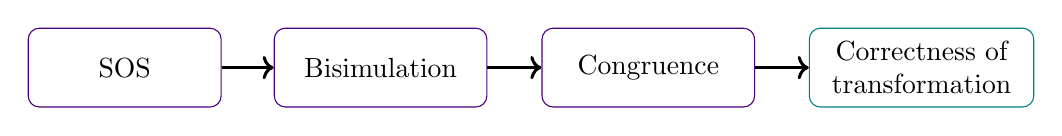
\begin{tikzpicture}[x=1cm,y=1cm]
    \node[draw=Indigo,rounded corners,minimum width=2.45cm,minimum height=1.0cm] (sos) at (0,0) {SOS};
    \node[draw=Indigo,rounded corners,minimum width=2.7cm,minimum height=1.0cm] (lts) at (3.25,0) {Bisimulation};
    \node[draw=Indigo,rounded corners,minimum width=2.7cm,minimum height=1.0cm] (cong) at (6.65,0) {Congruence};
    \node[draw=Teal,rounded corners,minimum width=2.85cm,minimum height=1.0cm,align=center] (corr) at (10.12,0) {Correctness of\\transformation};
    \draw[->,line width=1.1pt] (sos)--(lts);
    \draw[->,line width=1.1pt] (lts)--(cong);
    \draw[->,line width=1.1pt] (cong)--(corr);
  \end{tikzpicture}
  \vspace{7mm}
  \begin{exampleblock}{}
    Algebraic equations make proofs compact.\\[2mm]
    Bisimulations make them local.\\[2mm]
    Congruences make them reusable.\\[2mm]
    Simulations scale the idea to verified compilers.
  \end{exampleblock}
  \note{End with the distinction: process algebra was the training ground; realistic compiler proofs use state relations and one-way refinements.}
\end{frame}

\section{References}
% 44
\begin{frame}{References and suggested reading}
  \small
  \begin{thebibliography}{CompCert}
    \bibitem[MCS]{MCS}
      R. J. van Glabbeek.
      \emph{Modelling Concurrent Systems: Course Notes}.
      \newblock\href{https://homepages.inf.ed.ac.uk/rvangla/MCS/notes.html}{CCS expansion theorem and equational laws}.
    \bibitem[Milner]{Milner}
      R. Milner. \emph{Communication and Concurrency}.
      Prentice Hall, 1989.
    \bibitem[Leroy 2009]{Leroy}
      X. Leroy. \emph{Formal Verification of a Realistic Compiler}.
      Communications of the ACM 52(7), 2009.
    \bibitem[CompCert]{CompCert}
      \emph{CompCert 3.18 documentation}, August 2026.
      \newblock\href{https://compcert.org/man/manual001.html}{Manual},
      \href{https://compcert.org/doc/html/compcert.backend.Deadcodeproof.html}{dead-code proof},
      \href{https://compcert.org/doc/html/compcert.driver.Compiler.html}{whole-compiler proof}.
  \end{thebibliography}
  \note{The notes and CompCert proofs are public; links refer to precise statements and SOS rules.}
\end{frame}

\appendix
\inbackuptrue
\section{Optional material}
% A1
\begin{frame}{\optional State definitions for the optimisation proof}
  Let $\sigma_1=\sigma[x\mapsto1]$ and $\sigma_2=\sigma[x\mapsto2]$.
  \small
  \begin{align*}
  S_0&=\Store{x:=1;\,x:=2;\,\mathsf{out}(x);\,\mathsf{stop}}{\sigma},\\
  S_1&=\Store{x:=2;\,\mathsf{out}(x);\,\mathsf{stop}}{\sigma_1},\\
  S_2&=\Store{\mathsf{out}(x);\,\mathsf{stop}}{\sigma_2},\\
  S_3&=\Store{\mathsf{stop}}{\sigma_2},\\[1mm]
  T_0&=\Store{x:=2;\,\mathsf{out}(x);\,\mathsf{stop}}{\sigma},\\
  T_1&=\Store{\mathsf{out}(x);\,\mathsf{stop}}{\sigma_2},\\
  T_2&=\Store{\mathsf{stop}}{\sigma_2}.
  \end{align*}
  \note{Put this slide on the board or include it in the handout; it backs up the abbreviated state names on main proof slides.}
\end{frame}

% A2
\begin{frame}{\optional Complete bisimulation check}
  \small
  \renewcommand{\arraystretch}{1.35}
  \begin{tabular}{@{}p{.17\textwidth}p{.38\textwidth}p{.39\textwidth}@{}}
    \toprule
    Pair & Left transition & Right matching transition\\
    \midrule
    $(S_0,T_0)$ & $S_0\step{\tau}S_1$ & $T_0\step{\tau}T_1$\\
    $(S_1,T_1)$ & $S_1\step{\tau}S_2$ & $T_1\wstep{\tau}T_1$ (zero steps)\\
    $(S_2,T_1)$ & $S_2\step{\operatorname{out}(2)}S_3$ & $T_1\step{\operatorname{out}(2)}T_2$\\
    $(S_3,T_2)$ & $S_3\step{\mathsf{halt}}\nil$ & $T_2\step{\mathsf{halt}}\nil$\\
    $(\nil,\nil)$ & none & none\\
    \bottomrule
  \end{tabular}
  \vspace{2mm}
  \begin{block}{Reverse-direction obligations}
    The only nontrivial case is $T_1\step{\operatorname{out}(2)}T_2$
    from $(S_1,T_1)$: match it by
    $S_1\step{\tau}S_2\step{\operatorname{out}(2)}S_3$.
  \end{block}
  \note{This table plus the reverse-direction check proves that R is a weak bisimulation, for all initial stores.}
\end{frame}

% A3
\begin{frame}{\optional A stuttering forward simulation needs progress}
  \begin{block}{A potential pitfall}
    If one source step may be matched by \emph{zero} target steps indefinitely, an infinite source execution could collapse to a finite target execution.
  \end{block}
  \begin{exampleblock}{Standard repair}
    Add a well-founded measure decreasing on stuttering cases, or prove another suitable progress/divergence condition.
  \end{exampleblock}
  \Takeaway{A picture of matching finite prefixes is not the entire compiler-correctness theorem.}
  \Source{CompCert, \href{https://compcert.org/doc/html/compcert.common.Smallstep.html}{Smallstep: simulation relations and conversion theorems}.}
  \note{Do not identify the simple relation in the toy proof with the full mechanised forward_simulation record.}
\end{frame}

% A4
\begin{frame}{\optional Additional exercise: is this rewrite safe?}
  Consider
  \[
    \blockact{\{a,\bar a\}}{a.b.\nil\parallel\bar a.c.\nil}.
  \]
  \begin{enumerate}\setlength\itemsep{3mm}
    \item Compute its normal form without $\parallel$ or $\operatorname{block}$.
    \item Give a bisimulation relating the original and resulting LTSs.
    \item Would the equation remain valid if we blocked each component \emph{before} composing?
  \end{enumerate}
  \vspace{2mm}
  \Takeaway{Answer: $\tau.(b.c.\nil+c.b.\nil)$; the alternative blocking order is unsound.}
  \note{An appropriate 10-minute tutorial exercise. Do not use during a tight 90-minute lecture unless time remains.}
\end{frame}

\end{document}
